\documentclass[]{article}
\usepackage[utf8]{inputenc}
\usepackage{pdfpages}
\usepackage{amsmath}
\usepackage{amssymb}
\usepackage{graphicx}
\usepackage{geometry}
\usepackage{enumitem}
\usepackage{amsthm}

\usepackage{graphicx}
\usepackage{geometry}

\geometry{hmargin=2cm}

\title{Analyse}

\author{Isabelle Galagher et Pierre Gervais}
% Environnement type théorème
\newtheorem{mythm}{Théorème}
\newtheorem{myproposition}{Proposition}
\newtheorem{myproperty}{Propriété}
\newtheorem{mylemma}{Lemme}
\newtheorem{mycor}{Corollaire}

% Environnement type texte
\theoremstyle{remark}
\newtheorem{mynot}{Notation}
\newtheorem{myrem}{Remarque}
\newtheorem{myexer}{Exercice}
\newtheorem{myproof}{Preuve}
\newtheorem{myexmpl}{Exemple}

% Environnement de définition
\theoremstyle{definition}
\newtheorem{mydef}{Définition}

\setlist[itemize]{label=-}

% Carré de fin de preuve
\newcommand{\cqfd}{
	\hfill$\square$
}

% "Checkmark" de fin d'étape de preuve
\newcommand{\checked}{
	\hfill$\checkmark$
}

% Définition de fonction
\newcommand{\func}[5]{
#1 \, : \, \left\{ \begin{array}{lcl}
	#2 & \longrightarrow & #3 \\
	#4 & \longmapsto & #5
\end{array}
\right.
}

\newcommand{\funcinline}[5]{
#1 \, : \, #2 \longrightarrow #3, ~ #4 \longmapsto #5
}

\newcommand{\funcshort}[3]{
#1 \, : \, #2 \longrightarrow #3
}

\newcommand{\anonfunc}[4]{
\left\{ \begin{array}{lcl}
	#1 & \longrightarrow & #2 \\
	#3 & \longmapsto & #4
\end{array}
\right.
}

\newenvironment{proofpart}[1]{
	\noindent
	{\textbf{\boldmath #1}}
}{
	\checkmark
}

\newcommand*{\ClGa}[2]%
{\ensuremath{%
    #1/\!\raisebox{-.65ex}{\ensuremath{\mathcal{#2}}}}}

\newcommand*{\ClDr}[2]%
{\ensuremath{%
    \raisebox{-.65ex}{\ensuremath{#2}}\backslash #1}}

\begin{document}

\maketitle

\tableofcontents

\part{Topologie des espaces vectoriels normés}

On considèrera aussi les corps $\mathbb{R}$ ou $\mathbb{C}$

\section{Espaces vectoriels normés : premières définitions}

\subsection{Distances et normes}

\begin{mydef}
	Étant donné un ensemble $E$, une \textit{distance sur $E$} est une application $d~: ~ E \times E \longrightarrow \mathbb{R}$ vérifiant les propriétés suivantes :
	\begin{enumerate}
		\item $d$ est \textit{définie positive} : $d(x,y) \geqslant 0$ et $d(x,y) = 0 \Leftrightarrow x=y$
		\item $d$ est symétrique : $d(x,y)=d(y,x)$
		\item $d$ vérifie l'\textit{inégalité triangulaire} : $\forall z \in E, ~ d(x,y) \leqslant d(x,z) + d(z, y)$
	\end{enumerate}
\end{mydef}

\begin{myexmpl}
	\leavevmode
	\begin{itemize}
		\item $E=\mathbb{R}$ et $d(x, y) = |x-y|$
		\item $E=\mathbb{R}^2$ et $d\left(\binom{a}{b},\binom{c}{d}\right)=\sqrt{(a-c)^2+(b-d)^2}$
	\end{itemize}
\end{myexmpl}

\begin{myrem}
	Par l'inégalité triangulaire, on déduit
	\begin{itemize}
		\item $d(x,z) \geqslant d(x, y) - d(y, z)$
		\item $d(x, z) \geqslant d(z, y) - d(x, y)$
	\end{itemize}
	d'où $|d(x, y) - d(z, y)| \leqslant d(x, z)$
\end{myrem}

\begin{mydef}
	Soit $E$ un $\mathbb{K}$-espace vectoriel, une \textit{norme} sur $E$ est une application notée $N$ ou $\|\cdot\|$ telle que
	\begin{enumerate}
		\item $(x, y) \longmapsto \|x - y\|$ est une distance
		\item $\forall \lambda \in \mathbb{R}, ~ \forall u \in E, ~ \|\lambda u\| = |\lambda|\|u\|$ (\textit{homogénéité})
	\end{enumerate}
\end{mydef}

\begin{myproposition}
	Une fonction $\|\cdot\| ~ : ~ E \longrightarrow \mathbb{R}$ est une norme si et seulement si :
	\begin{enumerate}
		\item elle est homogène
		\item elle est définie
		\item elle vérifie l'inégalité triangulaire
	\end{enumerate}
\end{myproposition}

\begin{myproof}
	\leavevmode
	
	{\boldmath $\Longrightarrow$}
	
	Soit $\|\cdot\|$ une norme.
	\begin{enumerate}
		\item \checkmark
		\item $\|x\|=d(x, 0)$ où $d(x,y)=\|x-y\|$, donc $\|x\| \geqslant 0$ et $\|x\|=0 \Longleftrightarrow d(x, 0)=0 \Longleftrightarrow x=0$
		\item $\|x+y\| = d(x+y, 0) = d(x, -y)$, or $\forall x, y, z \in E, ~ d(x, z) \leqslant d(x, y) + d(y, z)$ donc $d(x, -y) \leqslant d(x, 0) + d(0, -y)$
		D'où $\|x+y\| \leqslant d(x, 0) + d(0, -y) \leqslant \|x\| + \|-y\| \leqslant \|x\| + \|y\|$
	\end{enumerate}
	
	{\boldmath $\Longleftarrow$}
	
	Soit $\| \cdot \|$ vérifiant les trois propriétés, alors soit $d(x, y)=\|x-y\|$ et montrons que d est une distance.
	
	\begin{enumerate}
		\item $d(x, y) \geqslant 0$ car $\|x-y\| \geqslant 0$ par (2).
		$d(x, y) = 0 \Longleftrightarrow \|x-y\| = 0 \Longleftrightarrow x = y$
		
		\item $d(x, y) = \|x-y\|=\|-(x-y)\| = \|y-x\|=d(y, x)$
		
		\item $d(x, y) = \|x-y\| = \|x-z + z - y\| \leqslant \|x-z\| +\|z-x\| \leqslant d(x, y) + d(z, y)$
 	\end{enumerate}
 	\cqfd
\end{myproof}

\begin{myexmpl}
	\leavevmode
	\begin{enumerate}
		\item Dans $\mathbb{R}^n$, on définit les normes $\displaystyle \|x\|_1= \sum_{k=1}^n |x_k|$, $\displaystyle \|x\|_2 =  \sqrt{\sum_{k=1}^n |x_k|^2}$, $\displaystyle \|x\|_p = \sqrt[p]{\sum_{k=1}^n |x_k|^p}$ et $\displaystyle \|x\|_\infty = \max_{k} \|x_k\|$
		\item Dans $\mathbb{R}^n$ muni d'un produit scalaire, $\|x\| = \sqrt{\langle x, x\rangle}$
		\item Soit $A$ un ensemble et $F$ une espace vectoriel normé, et $\mathcal{B}(A, F)$ les fonctions bornées de $A$ dans $F$, alors $\displaystyle \|f\|_\infty = \sup_{x \in A} \|f(x)\|$ est une norme.
		\item Sur $\mathcal{C}([0, 1], \mathbb{R})$, $\displaystyle \|f\|_1 = \int_{0}^{1}\left|f(x)\right|$, $\displaystyle \|f\|_2 = \sqrt{\int_{0}^{1}\left|f(x)\right|^2}$ et$\displaystyle \|f\|_\infty = \sup_{0 \leqslant x \leqslant 1}\left|f(x)\right|$
	\end{enumerate}
\end{myexmpl}

\begin{mydef}
	Deux normes $N_1$ et $N_2$ sont dites \textit{équivalentes} s'il existe des constantes strictement positives $C_1$ et $C_2$ telles que $\forall x \in E, ~ C_1 N_2(x) \leqslant N_1(x) \leqslant C_2 N_2(x)$
\end{mydef}

\begin{myexmpl}
	Par exemple dans $\mathbb{R}^n$, les normes $\|\cdot\|_1$, $\|\cdot\|_2$ et $\|\cdot\|_\infty$ sont équivalentes. En effet $$\|x\|_1=|x_1|+|x_2| \leqslant 2 \|x\|_\infty$$ et $\|x_i| \geqslant \|x\|_\infty, ~ i=1, 2$
\end{myexmpl}

En dimension finie, toutes les normes sont équivalentes ! Cela n'est en revanche pas vraie en dimension infinie.

\begin{figure}[h!]
	\centering
	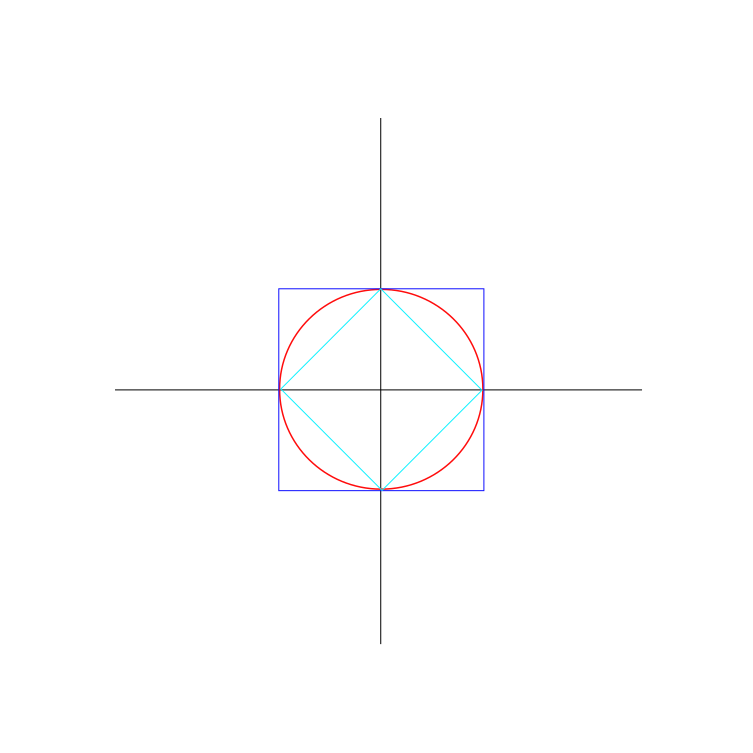
\includegraphics[width=350pt]{Schema1}
	\caption{Différentes boules unités}
	En bleu : $\mathcal{B}_\infty(0, 1)$
	
	En rouge : $\mathcal{B}_2(0, 1)$
	
	En turquoise : $\mathcal{B}_1(0, 1)$
\end{figure}

\subsection{Ouverts et fermés}

\begin{mydef}
	Soit $E$ un espace vectoriel normé, on appelle \textit{boule fermée} de centre $x$ et de rayon $r > 0$ l'ensemble $\overline{\mathcal{B}}(x, r) = \{u \in E ~|~ \|x-u\| \leqslant r\}$, et la \textit{boule ouverte} de centre $x$ et de rayon $r > 0$ l'ensemble $\mathcal{B}(x, r) = \{u \in E ~|~ \|x-u\| < r\}$.
\end{mydef}

\begin{mydef}
	Soit $X \subseteq E$
	\begin{enumerate}
		\item On dit que $U \subseteq X$ est un \textit{ouvert} de $X$ si $\forall x \in U, ~ \exists r > 0 ~ : ~ \mathcal{B}(x, r) \cap X \subseteq U$
		\item On dit que $F \subseteq X$ est un \textit{fermé} de $X$ si son complémentaire dans $X$ est un ouvert de $X$.
	\end{enumerate}
\end{mydef}

\begin{figure}[h!]
	\centering
	\includegraphics[width=200pt]{Ouverts_fermes}	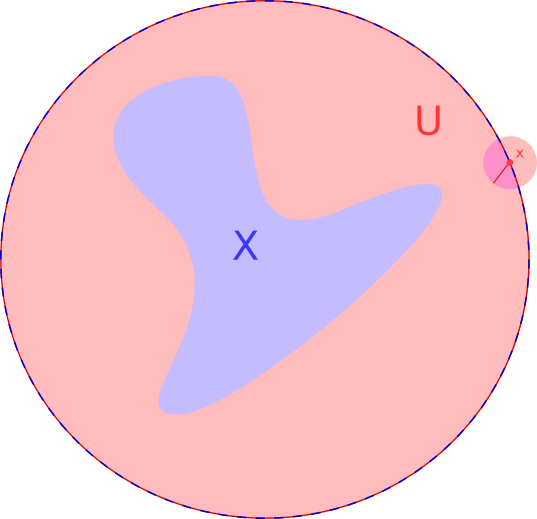
\includegraphics[width=200pt]{Ouverts_fermes2}
	\caption{Deux exemples d'ouverts}
\end{figure}

\begin{myrem}
	\leavevmode
	\begin{enumerate}
		\item Un ouvert dans $X$ n'est pas nécessairement ouvert dans $E$, comme montré dans le deuxième exemple de la figure ci-dessus.
		\item Un ouvert de $E$ sera appelé un \textbf{ouvert}, de même pour les fermés.
		
		\item Toute boule ouverte est un ouvert.
		
		\item Toute boule fermée est un fermé.
	\end{enumerate}
\end{myrem}

\newpage

\begin{myproof}
	On considère une boule ouverte $\mathcal{B}(x_0, r)$, montrons que c'est un ouvert.
	
	Soit $x \in \mathcal{B}(x_0, r)$, alors $\|x-x_0\| < r$. On cherche $r'$ tel que $\mathcal{B}(x, r') \subseteq \mathcal{B}(x_0, r)$ donc $r'$ doit vérifier $$\|x-y\| < r' \Longrightarrow \|x_0-y\| < r$$.
	
	Mais $\|x_0-y\| \leqslant \|x-y\| + \|x-x_0\| < \|x-y\| + r$.
	
	Soit $\delta = r - \|x-x_0\| > 0$, on pose alors $r'=\frac{\delta}{2} > 0$, alors $\|x_0-y\| \leqslant r' + \|x-x_0\| \leqslant r' + r - \delta < r$

	\cqfd
\end{myproof}

\begin{figure}[h!]
	\centering
	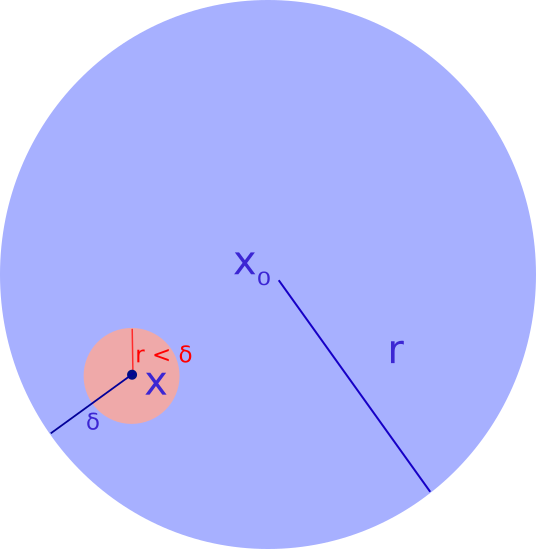
\includegraphics[width=350pt]{Schema2}
	\caption{Construction de la boule ouverte}
\end{figure}

\begin{myproposition}
	L'intersection de deux ouverts est un ouvert et toute réunion d'ouverts est un ouvert.
\end{myproposition}

\begin{myproof}
	Soient $U$ et $U'$ deux ouverts, montrons que $U \cap U'$ est un ouvert.
	
	Soit $x \in U \cap U'$, il existe $r>0$ et $r'>0$ tels que $\mathcal(B)(x, r) \subseteq U$ et $\mathcal{B}(x, r') \subseteq U'$.

	On pose $\widetilde{r}=\min(r, r')$ et on a $\mathcal{B}(x, \widetilde{r}) \subseteq U \cap U'$
	
	\cqfd
\end{myproof}

\begin{myproof}
	Soit $(U_i)_{i \in I}$ une famille d'ouverts, montrons que $U = \displaystyle \bigcup_{i \in I} U_i$ est un ouvert.
	
	Soit $x \in U$, alors il existe $i_0 \in I$ tel que $x \in U_{i_0}$, il existe donc $r$ tel que $\mathcal{B}(x, r) \subseteq U_{i_0}$ car $U_{i_0}$ est ouvert, d'où $\mathcal{B}(x, r) \subseteq U$.
	
	\cqfd
\end{myproof}

\begin{myproposition}
	Soit $X \subseteq E$, tout ouvert $U$ de $X$ s'écrit sous la forme $U=X \cap \widetilde{U}$, où $\widetilde{U}$ est un ouvert.
	
	De même pour tout fermé $F$ de $X$ s'écrit $F=X \cap \widetilde{F}$ où $\widetilde{F}$ est un fermé.
\end{myproposition}

\begin{myproof}
	Soit $\widetilde{U}$ un ouvert de $E$, alors $\widetilde{U} \cap X$ est un ouvert de $X$ par construction.
	
	Inversement soit $U$ ouvert de $X$, alors $\forall x \in U, ~ \exists r(x) > 0$ tel que $\mathcal{B}(x, r(x)) \cap X \subseteq U$
	
	Soit alors $\displaystyle \widetilde{U} = \bigcup_{x \in U} \mathcal{B}(x, r(x))$, alors $\widetilde{U}$ est un ouvert et $U = X \cap \widetilde{U}$
	\cqfd
\end{myproof}

\begin{mydef}
	Une suite à valeurs dans $E$ est dite \textit{convergente vers $x \in E$} si pour tout $\varepsilon > 0$ il existe un rang $N$ tel que pour tout $n \geqslant N$ on ait $\|x_n-x\| < \varepsilon$.
	
	Celle-ci est unique et on la note $\lim\limits_{n} x_n = x$.
\end{mydef}

On remarquera qu'une suite convergente est bornée.

\begin{myproof}
	Soient $x$ et $y$ deux limites de la suite convergente $(x_n)_n$.
	
	Pour tout $\varepsilon > 0$ on peut trouver un rang $N$ à partir duquel $\|x_n-x\|<\varepsilon$ et $\|y_n-x\|<\varepsilon$, d'où
	
	$$\|x-y\| \leqslant \|x-x_n\| + \|x_n-y\| < 2\varepsilon$$
	
	Cette inégalité est vraie pour tout $\varepsilon>0$ donc $x=y$.
	
	\cqfd
\end{myproof}

\begin{myrem}
	On rappelle que dans $\mathbb{R}$, toute suite majorée croissante est convergente.
	
	Soit $A=\{x_n ~ | ~ n \geqslant 0\}$, et on note $l = \sup A$.
	
	Soit $\varepsilon > 0$, $l - \varepsilon$ ne majore pas $A$ donc il existe un rang $N$ à partir duquel $x_n \geqslant l-\varepsilon$, mais on a aussi $x_n \leqslant l$ pour tout $n$, on a ainsi à partir de $N$ l'encadrement $l - \varepsilon \leqslant x_n \leqslant l + \varepsilon$.
	
	On a de plus que $\lim\limits_{n} x_n = \sup \{x_n | n \geqslant 0\}$
\end{myrem}

\begin{myrem}
	Si une suite est convergente pour une norme, alors elle l'est pour toute norme équivalente à celle-ci.
	
	Cela n'est pas vrai en général si les normes ne sont pas équivalentes.
	
	Sur l'ensemble des fonctions continue sur $[0, 1]$ on définit les normes
	
	$$\|f\|_{\infty} = \sup_{[0,1]} |f(x)| \text{ et } \|f\| = \int_{0}^{1} |f|$$
	
	On considère la suite de fonction $f_n ~ : ~ x \longmapsto x^n$, on a $$\displaystyle \|f_n\|_{\infty} = \sup_{[0, 1]} |f_n(x)| = 1$$ mais $\|f_n\|=\int_{0}^{1}x^ndx=\frac{1}{n+1} \longrightarrow 0$, les normes ne sont pas équivalentes.
\end{myrem}

\begin{mydef}
	On appelle \textit{valeur d'adhérence} de $x_n$ toute limite d'une sous-suite (suite extraite) de $(x_n)$.
	
	Et on appelle \textit{point d'accumulation} d'une suite $(x_n)$ un point $x$ tel que $\forall \varepsilon > 0, ~ \forall N, ~ \exists n > N ~ : ~ \|x_n-x\| < \varepsilon$.
\end{mydef}

\begin{myproposition}
	Tout point d'accumulation d'une suite convergente $(x_n)$ est une valeur d'adhérence, et réciproquement.
\end{myproposition}

\begin{myproof}
	\begin{proofpart}{Valeur d'adhérence $\Longrightarrow$ point d'accumulation :}
	
		Soit $x$ une valeur d'adhérence de $(x_n)$, il existe une fonction entière strictement croissante $\varphi$ telle que $$\forall \varepsilon > 0, ~ \exists N ~ : ~ \forall n > N, ~ \|x_{\varphi(n)}-x\| < \varepsilon$$
		donc $x$ est un point d'accumulation.
	\end{proofpart}
	
	\begin{proofpart}{Point d'accumulation $\Longrightarrow$ valeur d'adhérence :}
		Réciproquement, soit $x$ un point d'accumulation d'une suite $(x_n)$, on construit par récurrence $\varphi$ telle que $x$ soit la limite de $(x_{\varphi(n)})_n$ par 
		
		$$
		\varphi(n) = \left\{
			\begin{array}{ll}
				0, ~ n = 0 \\
				\min\{k > \varphi(n-1) ~ | ~ \|x_k-x\| < 2^{-n}\}, ~ n > 0
			\end{array}
		\right.
		$$
		
		L'application est bien strictement croissante.
		
		Montrons à présent que $y_n=x_{\varphi(n)}$ converge vers $x$ : 
		
		soit $\varepsilon \in ]0, 1[$, on cherche $N$ tel que pour tout $n > N, ~ \|x_n-x\| < \varepsilon$.
		
		Pour $N > \frac{\ln \varepsilon}{\ln 2}$ on a $$\forall n > N, ~ \|y_n-x\| < 2^{-n} < \varepsilon$$
		
		$(y_n)_n$ est bien une suite convergeant vers $x$.
	\end{proofpart}
	
\end{myproof}

\begin{myproposition}
	Soit $E$ un espace vectoriel normé et $F \subseteq E$.
	
	F est fermé \textit{si et seulement si} $F$ contient la limite de toutes ses suites convergentes.
\end{myproposition}

\begin{myproof}
	\begin{proofpart}{$F$ fermé $\Longrightarrow$ $F$ contient les limites de ses suites}

		Soit $(x_n)$ une suite convergente de $F$ de limite $x$. Montrons que $x \in F$.
		
		Supposons par l'absurde $x \not \in F$, alors $x \in F^C$ qui est ouvert. Il existe donc $r > 0$ tel que $\mathcal{B}(x, r) \subseteq (E \verb|\|F)$, mais il existe un rang à partir duquel $\|x_n-x\| < \frac{r}{2}$, c'est à dire $x_n \in \mathcal{B}(x, r)$, ce qui contredit $\mathcal{B}(x, r) \subseteq F^C$.
	\end{proofpart}
	
	
	\begin{proofpart}{$F$ contient les limites de ses suites $\Longrightarrow$ $F$ est fermé}
		Montrons que $F^C$ est fermé, ce qui est est équivalent au fait que $F$ soit fermé.
		Soit $u \in F^C$, on pose $r=\inf\limits_{f \in F} \|f-u\|$.
		
		Supposons par l'absurde que $r$ soit nul, alors pour tout $n>0$ il existerait un élément $f_n \in F$ tel que $\|u-f_n\| < \frac{1}{n}$. Cela définit alors une suite $(f_n)_n$ à valeurs dans $F$ convergente vers $u \notin F$, ce qui contredit le fait que $F$ contienne ses limites.
		
		On a alors $\mathcal{B}_r(u) \subseteq F^C$, $F^C$ est donc effectivement ouvert.
	\end{proofpart}
	\begin{figure}[h!]
		\centering
		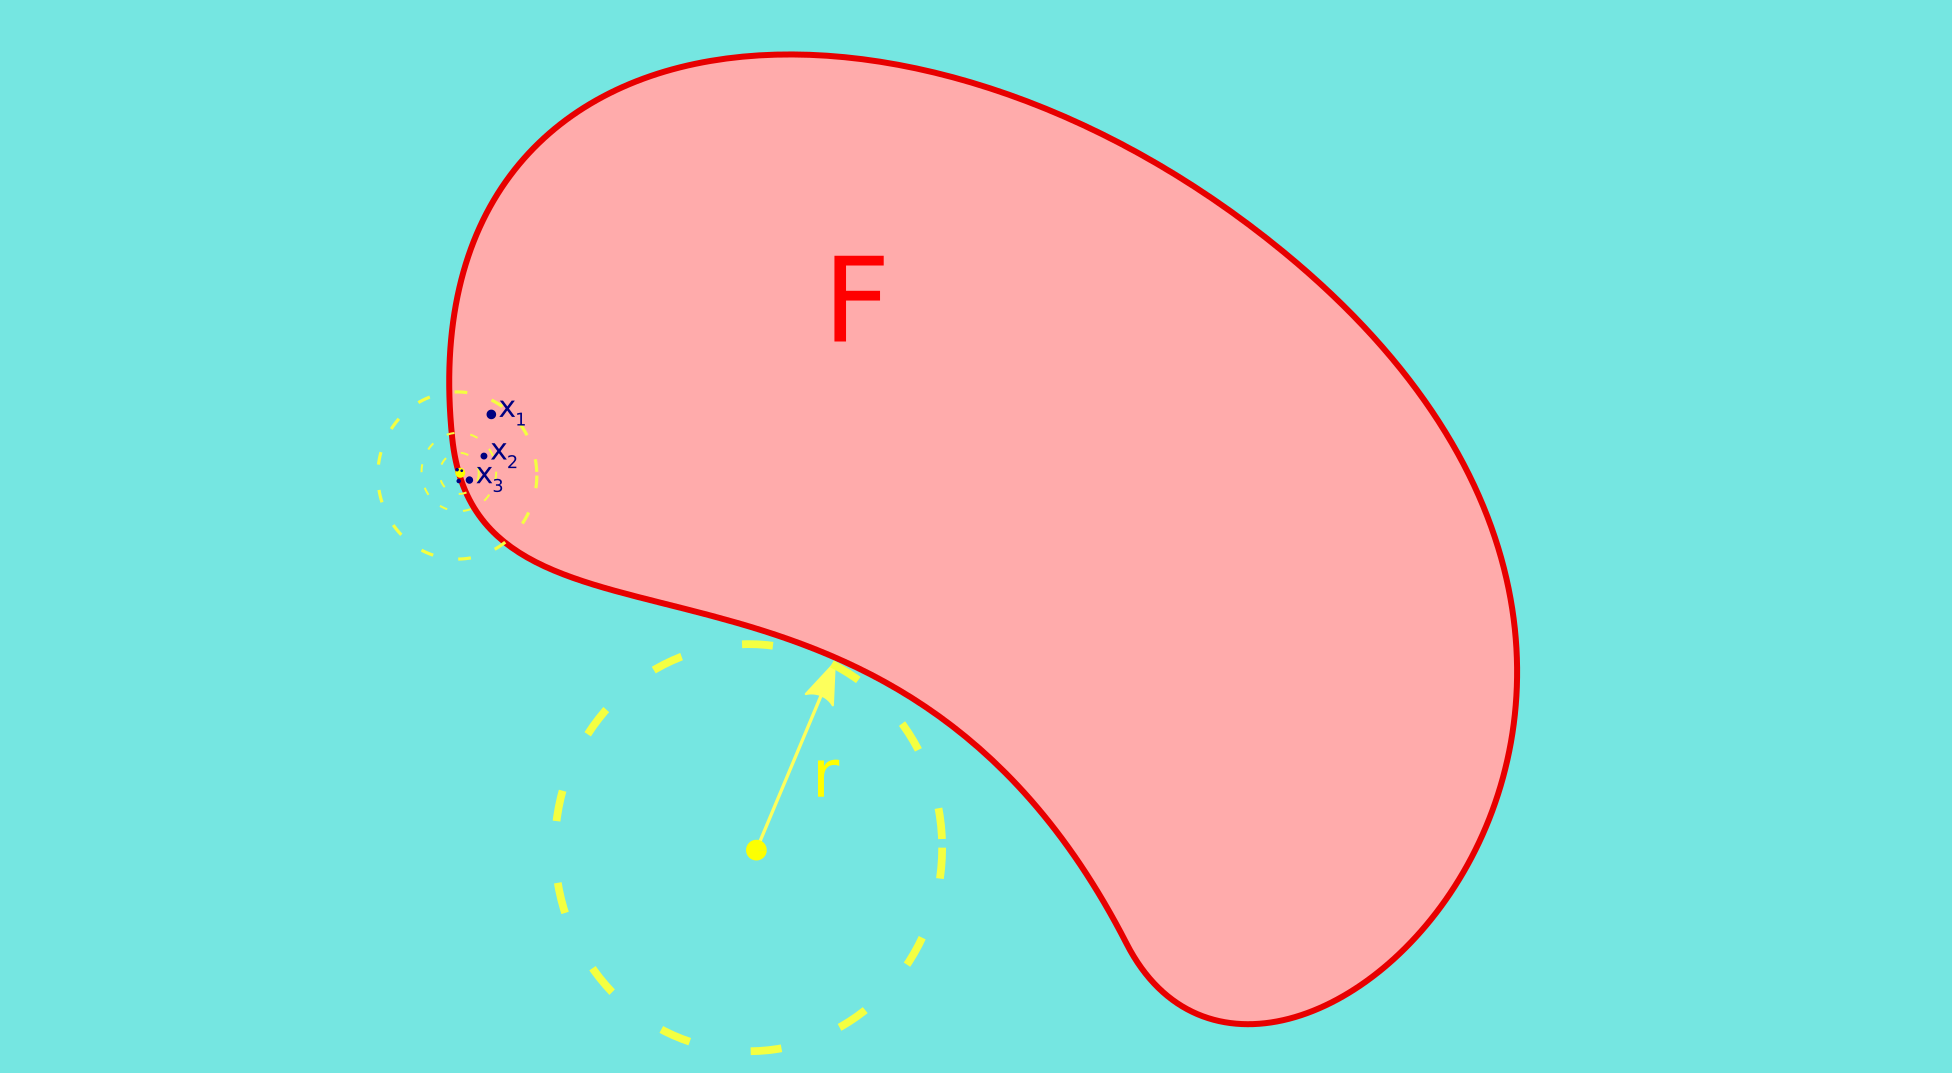
\includegraphics[width=450pt]{Contient_ses_limites_implique_ferme}
		\caption{Une partie contenant ses limites est fermée}
		
		Si on avait $r=\inf\limits_{f \in F} \|u-f\|=0$, alors on aurait $u \in F$ car toute boule ouverte centrée en $u$ s'intersecterait avec le fermé $F$. 
	\end{figure}	
	\cqfd
\end{myproof}

\begin{mydef}
	Soit $X$ une partie d'un espace vectoriel normé $E$.
	
	\begin{itemize}
	\item \textit{L'intérieur de $X$} est le plus grand ouvert inclus dans $X$ noté $\mathring{A}$.
	
	\item \textit{L'adhérence de $X$} est le plus petit fermé contenant $X$ noté $\overline{X}$.
	
	\item \textit{La frontière de $X$} est l'ensemble $\partial X=Fr(X)=\overline{X} \verb|\| \mathring{X}$
	\end{itemize}
\end{mydef}

\begin{myexmpl}
	Si $X = ]0, 1]$ sur $\mathbb{R}$ alors $\mathring{X} = ]0, 1[$, $\overline{X}=[0, 1]$ et $Fr(X)=\{0, 1\}$.
\end{myexmpl}

\begin{myrem}
	X est ouvert si est seulement si $\mathring{X} = X$ et $X$ est fermé si et seulement si $\overline{X}=X$.
	
	En effet, pour $X$ ouvert, $\mathring{X}$ est le plus grand ouvert contenu dans $X$, donc $X$.
	
	Réciproquement si $X=\mathring{X}$, l'intérieur d'une partie étant un ouvert on a bien que $X$ est ouvert.
\end{myrem}

\begin{myproof}Intérieur
	
	Soit $\mathring{X}$ l'ensemble des $x \in X$ tels qu'il existe $r > 0$ tel que $\mathcal{B}(x, r) \subseteq X$, alors $\mathring{X}$ est la réunion de tous les ouverts contenus dans $X$.
	
	En effet, $\mathring{X}$ est ouvert dans $X$ par définiton, donc $\mathring{X} \subseteq \text{"réunion des ouverts de X"}$.
	
	Soit $U$ un ouvert de $X$, montrer que $U \subseteq X$.
	
	Soit $x \in U$, il existe $r>0$ tel que $\mathcal{B}(x, r) \subseteq U$ ar $U$ est ouvert. Donc $x \in \mathring{X}$.
	
	$\mathring{X}$ est donc ouvert, contenu dans $X$. Il contient tous les ouverts de $X$, donc c'est le plus grand de $X$, d'où le résultat.
	\cqfd
\end{myproof}

\begin{myproposition}
	On caractérise l'adhérence d'une partie $X$ comme étant l'ensemble des limites de sous-suites de $X$.
\end{myproposition}

\begin{myproof}
	Soit $A$ l'ensemble des limites de suites convergentes à valeurs dans $X$.
	
	
	\begin{proofpart}{$A$ est un fermé contenant $X$}
		Pour tout $x \in X$, $x$ peut être la limite d'une suite à valeur dans $X$, c'est à dire $x \in A$ et donc $X \subseteq A$.
		
		Cela signifie en particulier que $A$ contient les limites de ses suites : c'est un fermé.
	\end{proofpart}
	
	\begin{proofpart}{$A$ est le plus petit fermé contenant X}
	
	Montrons que $A$ est minimal, c'est-à-dire que pour tout fermé $F$ vérifiant $X \subseteq F \subseteq A$, on a $F=A$.
	
	$F$ est un fermé contenant $X$, donc il contient $X$ et les limites des suites convergentes à valeurs dans $X$, c'est à dire $A$.
	\end{proofpart}
	
	$A$ est donc le plus petit fermé contenant $X$, c'est à dire $A = \overline{X}$	
\end{myproof}

\section{Applications continues}

\begin{mydef}
	Soient $E$ et $F$ deux espaces vectoriels normés, soient $X \subseteq E$, $Y \subseteq F$ et $f$ une application de $X$ dans $Y$.
	
	On dit que $f$ est continue en un point $x \in X$ si $$\forall \varepsilon > 0, \exists \delta > 0 ~ : ~ (\forall u, ~ \|x-u\| < \delta \Longrightarrow \|f(x)-f(u)\| < \varepsilon)$$
\end{mydef}

\begin{mythm}
	Une application $f~:~X \longrightarrow Y$ est continue en $x_0 \in X$ si et seulement si pour toute suite $(y_n)$ convergeant vers $x_0$, la suite $\left(f(y_n)\right)_n$ converge vers $f(x_0)$.
\end{mythm}

\begin{myexer}
	Le démontrer
\end{myexer}

\begin{mythm}
	Soit une application $f~:~X \longrightarrow Y$, les assertions suivantes sont équivalentes :
	\begin{enumerate}
	 \item $f$ est continue sur $X$
	 \item l'image réciproque de tout ouvert de $Y$ est un ouvert de $X$
	 \item l'image réciproque de tout fermé de $X$ est une fermé de $X$.
 	\end{enumerate}
\end{mythm}

\begin{myproof}
	\begin{proofpart}{1. $\Longrightarrow$ 2.}
		Soit $f$ continue sur $X$ et $U$ un ouvert de $Y$. Montrer que $f^{-1}(U)=V$ est un ouvert de $X$.
		
		Soit $x \in f^{-1}(U)$, alors $f(x) \in U$, il existe donc $r>0$ tel que $\mathcal{B}(f(x), r) \subseteq U$.
		
		Or il existe $\delta > 0$ tel que pour $\|x-u\| < \delta$, on a $\|f(x)-f(y)\| < \frac{r}{2}$.
		
		Ainsi si $y \in \mathcal{B}\left(x, \frac{\delta}{2}\right)$ alors $f(y) \in \mathcal{B}(f(x), r) \subseteq U$, donc $y \in f^{-1}(U)$.
		
		$f^{-1}(U)$ est donc un ouvert.
	\end{proofpart}
	
	\begin{proofpart}{2. $\Longrightarrow$ 1.}
		Soit $\varepsilon > 0$, on veut trouver $\delta > 0$ tel que si $\|x-y\| < \delta$, alors $\|f(x)-f(y)\| < \varepsilon$.
	
		Soit $x \in X$, alors $\mathcal{B}_\varepsilon(f(x))$ est un ouvert de de $Y$, on sait que $f^{-1}(\mathcal{B}_\varepsilon(f(x)))$ est un ouvert de $X$ contenant $x$, il existe donc $\delta > 0$ tel que $\mathcal{B}_\delta(x) \subseteq f^{-1}(\mathcal{B}_\varepsilon(f(x)))$.
		
		Autrement dit, si $\|x-y\| < \delta$ alors $y \in f^{-1}(\mathcal{B}_\varepsilon(f(x)))$, c'est-à-dire $\|f(x)-f(y)\| < \varepsilon$.
	\end{proofpart}
	
	\begin{proofpart}{1. $\Longleftrightarrow$ 2.}
		On le démontre en passant au complémentaire.
	\end{proofpart}
	
	\cqfd
\end{myproof}

\begin{mycor}
	Soient $X \subseteq E$, $Y \subseteq F$ et $f$ une application de $X$ dans $Y$.
	\begin{enumerate}
		\item On suppose que $f$ est continue, alors la restriction de $f$ à $X' \subseteq X$ notée $f_{|X'}$ est continue.
		
		\item Si $X'$ est un ouvert de $X$ et si $f_{|X'}$ est continue alors $f$ est continue en tout point de $X'$.
		
		\item Soient $f$ et $g$  avec $\funcshort{f}{E}{F}$ et $\funcshort{g}{F}{G}$ avec $E, F, G$ des espaces vectoriels normés. Si $f$ et $g$ sont continues alors $g \circ f$ est continue.
	\end{enumerate}
\end{mycor}

\newpage

\begin{myrem}
	L'hypothèse que $X'$ soit ouvert est nécessaire pour le point 2.
	\begin{figure}[h!]
		\centering
		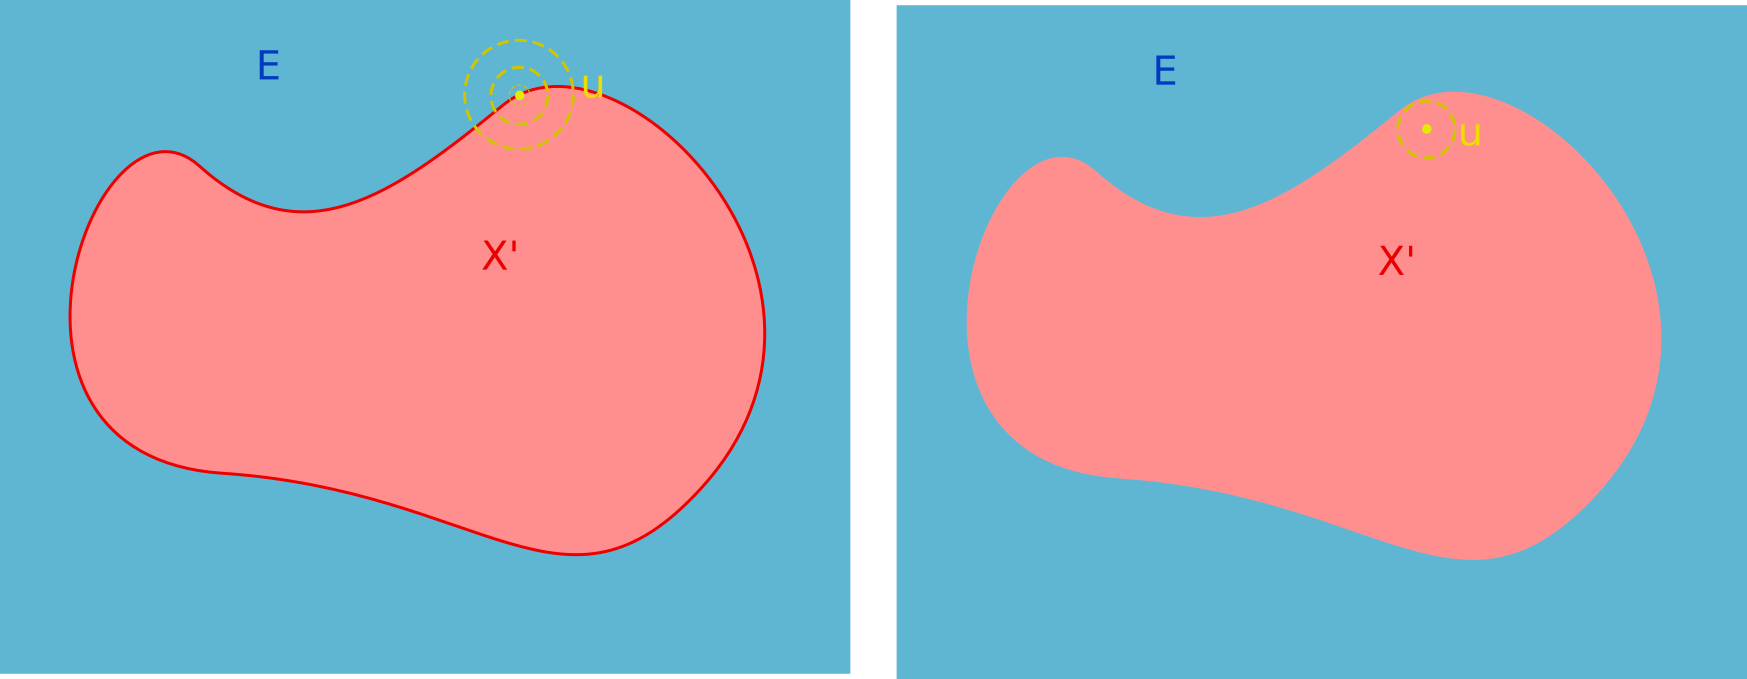
\includegraphics[width=550pt]{Application_continue}
		\caption{Restriction continue sur une partie non-ouverte ou ouverte}
		
		$\func{f}{\mathbb{R}^2}{\mathbb{R}}{u}{\text{rouge si } u \in X', ~ \text{ bleu sinon}}$
		
		\begin{itemize}
		\item A gauche, $f_{|X'}$ est continue mais $f$ n'est pas continue sur $X'$ car on ne peut pas trouver une boule ouverte de $X'$ autour du point $u$.
		
		\item A droite, on peut trouver une boule ouverte autour de $u$ car $X'$ est ouvert.
		\end{itemize}
	\end{figure}
\end{myrem}

\begin{myproof}
	\begin{proofpart}{Point 1.}
		Soit $X' \subseteq X$ et $V$ un ouvert de $Y$, montrons que $\left(f_{|X'}\right)^{-1}(V)$ est un ouvert de $X'$.
		
		$f$ est continue sur donc il existe $U$ ouvert de $E$ tel que $f^{-1}(V)= X \cap U$.
		
		Mais alors $\left(f_{|X'}\right)^{-1}(V) = X' \cap X \cap U = X' \cap U$ qui est un ouvert de $X'$.
		
		Donc $f_{|X'}$ est continue.
	\end{proofpart}
	
	\begin{proofpart}{Point 2.}
		$f_{|X'}$ est continue, soit $x \in X'$, montrons que $f$ est continue en $x$.
		
		Soit $\varepsilon > 0$, il existe $\delta
		 > 0$ tel que si $y \in X'$ et $\|x-y\| < \delta$ alors $\|f(x)-f(y)\| < \varepsilon$
		 
		 Comme $X'$ est ouvert, il existe $r > 0$ tel que $\mathcal{B}_r(x) \subseteq X'$.
		 
		 On choisit $\delta' \leqslant \min\{r, \delta\}$, alors $\forall y \in \mathcal{B}_{\delta'}, ~ \|f(x)-f(y)\| < \varepsilon$, donc $f$ est continue en $x$.
	\end{proofpart}
	
	\begin{proofpart}{Point 3.}
	\end{proofpart}
\end{myproof}


\section{Applications uniformément continues, applications linéaires continues}

\begin{mydef}
	Une application $\funcshort{f}{E}{F}$ est \textit{uniformément continue} si $$\forall \varepsilon, ~ \exists \delta > 0 ~ : ~ \forall x, y \in E, ~ (\|x-y\| < \delta \Longrightarrow \|f(x)-f(y\| < \varepsilon)$$
\end{mydef}

\begin{myrem}
	Si est uniformément continue alors elle est continue, la réciproque ets cependant fausse.
\end{myrem}

\begin{mydef}
	Une fonction $f$ est $k$-\textit{lipschitzienne} si
	
	$$\forall x, y \in E, ~ \|f(x)-f(y)\| \leqslant k \|x-y\|$$
\end{mydef}

\begin{mythm}
	Soit $\funcshort{\varphi}{E}{F}$ une application linéaire, alors les propriétés suivantes ont équivalentes :
	
	\begin{enumerate}
		\item $\varphi$ est continue
		\item $\varphi$ est continue en 0
		\item $\varphi$ est uniformément continue
		\item $\varphi$ est bornée sur $\mathcal{B}_1(0)$
		\item $\varphi$ est $k$-lipschitzienne.
	\end{enumerate}
\end{mythm}


\begin{myproof}
	Montrons $2. \Longrightarrow 4. \Longrightarrow 5. \Longrightarrow 3.\Longrightarrow 1. \Longrightarrow 2.$
	
	\begin{proofpart}{$1. \Longrightarrow 2.$}
	\end{proofpart}
	
	\begin{proofpart}{$2. \Longrightarrow 4.$}
		$f$ est continue en 0, donc pour tout $\varepsilon > 0$ il existe $\delta > 0$ tel que $\|x\| < \delta \Longrightarrow \|f(x)\| < \varepsilon$
		
		Soit $x \in \mathcal{B}_1(0)$ avec $x \neq 0$, on a :
		
		$$\|x\| < 1$$

		$$\|\delta x\| < \delta$$
		
		$$\|f(\delta \cdot x)\| < \varepsilon$$
		
		$$\|f(x)\| < \frac{\varepsilon}{\delta}$$
	\end{proofpart}
	
	\begin{proofpart}{$4. \Longrightarrow 5.$}
		Supposons que $f$ soit majoré par $M > 0$ sur la boule unité.
		
		Soient $x \neq y \in E$, on a
		$$x-y = (x-y) \cdot \frac{\|x-y\|}{\|x-y\|}$$
		
		$$f(x-y) = \|x-y\| f\underbrace{\left(\frac{x-y}{\|x-y\|}\right)}_{\in \mathcal{B}_1(0)}$$
		
		$$f(x-y) = \|x-y\| \cdot M$$
		
		$f$ est $M$-lipschitzienne.
	\end{proofpart}
	
	\begin{proofpart}{$5. \Longrightarrow 3. \Longleftarrow 1. \Longrightarrow 2.$}
	\end{proofpart}
\end{myproof}

\begin{mydef}
	Soit $f$ une application lipschitzienne, on appelle \textit{constante de Lipschitz de $f$} ou \textit{norme d'opérateur de $f$} la valeur $\|f\| = \inf \{k > 0 ~|~ f \text{ est }k \text{-liptschitzienne}\} = \sup\limits_{\|x\|=1} \|f(x)\| = \sup\limits_{\|x\| \leqslant1} \|f(x)\|$
\end{mydef}

La norme d'opérateur est comme son nom l'indique une norme, en particulier $$\forall x, y \in E, ~ \|f(x)\|\leqslant \|f\|\|x\|$$

\begin{myproposition}
	Soient $E$ et $F$ deux espaces vectoriels normés, o note $\mathcal{L}_C(E)$ l'ensemble des applications linéaires continues de $E$ dans $F$. C'est un espace vectoriel normé si on le munit de la norme d'opérateur.
	
	$$\forall \varphi, \psi \in \mathcal{L}_C(E, E), ~ \|\varphi \circ \psi\| \leqslant \|\varphi\| \|\psi\|$$
\end{myproposition}

\begin{myrem}
	On peut étendre ces résultats aux applications bilinéaires : soient $E$, $E'$ et $F$ trois espaces vectoriels normés, et $\funcshort{f}{E \times E'}{F}$ bilinéaire continue,sa norme d'opérateur est définie par
	$$\|f\| = \sup\{\|f(x, y)\| ~ | ~ \|x\| \leqslant 1, ~ \|y\| \leqslant 1\}$$
	
	On a en particulier $\|f(x,y)\| \leqslant \|f\| \cdot \|x\| \cdot \|y\|$
\end{myrem}

\section{Espaces produits}

\begin{mydef}
	Soient $(E_1, N_1)$ et $(E_2, N_2)$ deux espaces vectoriels normés, on construit des normes sur $E_1 \times E_2$ en posant
	$$\|(x, y)\|_1 = N_1(x) + N_2(y)$$
	$$\|(x, y)\|_2 = \sqrt{N_1^2(x) + N_2^2(y)}$$
	$$\|(x, y)\|_\infty = \max\{N_1(x), N_2(y)\}$$
\end{mydef}

On a les relations $$\|(x, y)\|_\infty \leqslant \|(x, y)\|_2 \leqslant \|(x, y)\|_1 \leqslant 2 \|(x, y)\|_\infty$$

\begin{myexmpl}
	Soit $E$ un espace vectoriel normé, on munit $E \times E$ de la norme définie par $N(x, y)=\|x\|+\|y\|$ et on définit une distance $d(u, v)=\|u-v\|$
	
	$d$ est lipschitzienne :
	$$|d(x, y) - d(x', y')|=|\|x-y\|-\|x'-y'\||$$
	
	$$|d(x, y) - d(x', y')| \leqslant |\|(x-y)-(x'-y')\||$$
	
	$$|d(x, y) - d(x', y')| \leqslant |\|(x-x')+(y'-y)\||$$

	$$|d(x, y) - d(x', y')| \leqslant \|(x-x')\|+\|(y'-y)\|$$
	
	$$|d(x, y) - d(x', y')| \leqslant N((x-x')+(y'-y))$$
	
	$d$ est donc 1-lipschitzienne.
\end{myexmpl}

\begin{myproposition}
	Soient $E_1$ et $E_2$ deux espaces vectoriels normés, alors :
	
	\begin{enumerate}
		\item Les projections $\func{\pi_1}{E_1 \times E_2}{E_1}{(x,y)}{x}$
		et $\func{\pi_2}{E_1 \times E_2}{E_1}{(x,y)}{y}$
		sont lipschitziennes.
		
		\item Une application $\funcshort{f}{Y}{E_1 \times E_2}$ notée $f=(f_1, f_2)$ avec $\funcshort{f_1}{Y}{E_1}$ et $\funcshort{f_2}{Y}{E_2}$ est continue si et seulement si $f_1$ et $f_2$ sont continues.
		
		\item Si $\funcshort{f}{E_1 \times E_2}{F}$ est continue alors pour tout $x \in E_1$, l'application $\func{f_x}{E_2}{F}{y}{f(x, y)}$ est continue et de même $\func{f_y}{E_1}{F}{x}{f(x, y)}$ est continue pour tout $y \in E_2$.
	\end{enumerate}
\end{myproposition}

\begin{myproof}
	\begin{enumerate}
		\item Soit $(x, y) \in E_1 \times E_2$, alors $\pi_1(x, y) = x$, donc $\pi_1(x,y) - \pi_2(x',y')=x'-y'$ et donc $\|\pi_1(x,y) - \pi_2(x',y')\| = \|x-x'\| \leqslant \|x-x'\| + \|y-y'\| = N_1(x-x', y-y')$
		
		$\pi_1$ est 1-lipschitzienne.
		
		\item Si $f$ est continue, alors $\pi_1 \circ f=f_1$ est continue comme composée d'applications continues.
		
		De même $f_2=\pi_2 \circ f$ est continue.
		
		Inversement, supposons que $\funcshort{f_1}{Y}{E_1}$ et $\funcshort{f_2}{Y}{E_2}$ sont continues.
		
		Montrons que $\func{f=(f_1, f_2)}{Y}{E \times E_2}{x}{(f_1(x), f_2(y)}$
		
		Soit $(x_n)_n$ une suite de $Y$ convergeant vers $x \in Y$, montrons que $(f(x_n))_n$ converge vers $f(x)$.
		
		Comme $f_1$ est continue, $(f_1(x_n))_n$ converge $f_1(x)$ et de même pour $f_2$.
		
		Donc $f(x_n)_n$ converge vers $f(x)=(f_1(x), f_2(x))$
		
		\item Se démontre de même par caractérisation séquentielle de la continuité.
	\end{enumerate}
\end{myproof}

\begin{myrem}
	Une fonction peut être continue de chaque variable sans être continue du couple de variables, par exemple
	$$f ~ : ~ \left\{
	\begin{array}{ccl}
		\mathbb{R}^2 & \longrightarrow & \mathbb{R} \\
		(x, y) & \longmapsto & \frac{xy}{x^2+y^2}, \text{ si } (x, y) \neq (0, 0) \\
		(0, 0) & \longmapsto & 0
	\end{array}
	\right.$$
	
	$f$ est continue pour $x$ et $y$ fixé, mais $\forall \varepsilon > 0, ~ f(\varepsilon, \varepsilon) = \frac{1}{2}$
	$f$ n'est donc pas continue car $f(0, 0)=0$.
	
		\begin{figure}[h!]
			\centering
			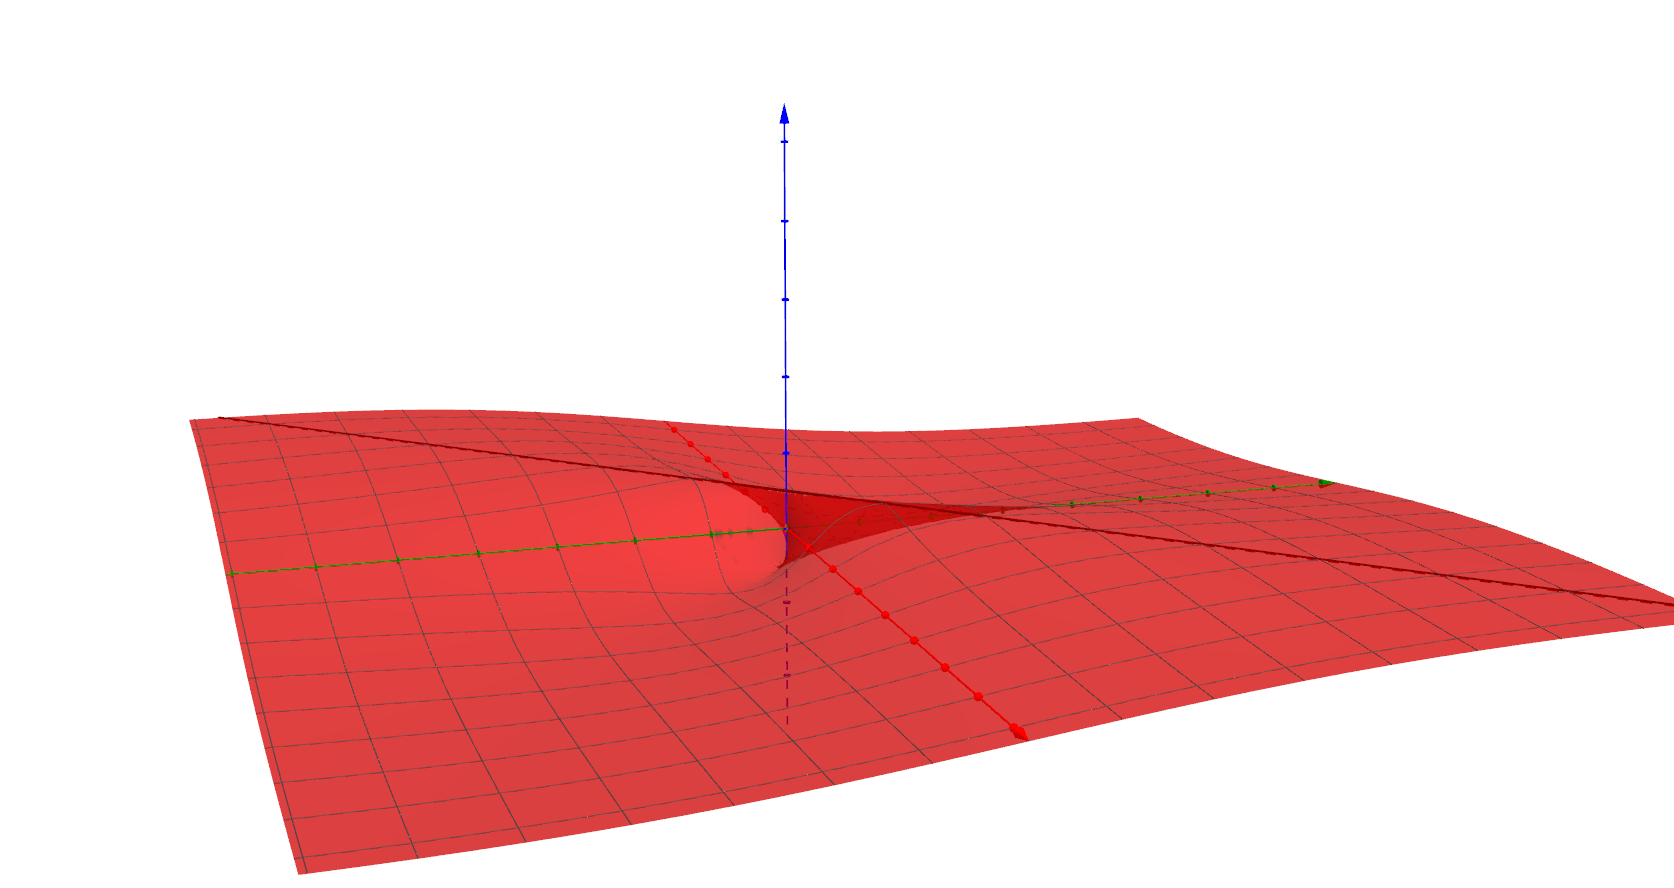
\includegraphics[width=550pt]{Continue_sur_chaque_variable}
			\caption{$\left(x, y, \frac{xy}{x^2+y^2}\right)$ et $(t, t, f(t, t))$}
		\end{figure}
\end{myrem}

\part{Compacité et complétude}

\section{Sous-suites et compacité}
	
\begin{mythm}{Bolzano-Weierstrass}

	Toute suite réelle bornée admet une sous-suite convergente.
\end{mythm}

\begin{myproof}
	Soit $(x_n)_n$ bornée par $M > 0$, on définit pour tout $n \geqslant 0$ l'ensemble $Y_n = \{x_k ~ | ~ k \geqslant n\}$ et $y_n=\sup Y_n$.
	
	On a alors pour tout $n$, $Y_{n+1} \subseteq Y_n$ et donc $y_{n+1} \leqslant y_n$.
	
	$(y_n)_n$ est donc une suite minorée par $-M$ décroissante, elle converge ainsi vers une limite $\ell = \inf \{y_n ~ | ~ n \geqslant 0\}$.
	
	Construisons une suite $(x_{k_n})_n$ à l'aide d'une suite strictement croissante $(k_n)_n$ d'entiers tels que :
	
	$$\forall n \geqslant 1, ~ |x_{k_n}-\ell| \leqslant \frac{1}{n}$$
	
	On choisit $k_0 = 1$ et on suppose avoir construit : $k_0, k_1, k_2, ..., k_{n-1}$.
	
	Par définition de la suite $(y_n)_n$, il existe un entier $p_n$ tel que : $$0 \leqslant y_{p_n} - \ell \leqslant \frac{1}{n}$$
	
	Mais $(y_k)_k$ est décroissante, alors $\forall k \geqslant p_n$ on a $0 \leqslant y_k - \ell \leqslant \frac{1}{n}$.
	
	$y_{p_n}$ étant une borne supérieure, il existe $k_n \geqslant p_n$ tel que $y_{p_n} - \frac{1}{n} \leqslant x_{k_n} \leqslant y_{p_n}$, ce qui donne :
	$$y_{p_n} - \ell - \frac{1}{n} \leqslant x_{k_n} - \ell \leqslant y_{p_n} - \ell$$
	
	En particulier on a : $$-\frac{1}{n}\leqslant x_{k_n}-\ell \leqslant \frac{1}{n}$$.
	
	\cqfd
\end{myproof}

\begin{mydef}
	Une partie de $X$ d'un espace vectoriel normé est \textit{compacte} si toute suite à valeurs dans $X$ admet une sous-suite convergente dans $X$.
\end{mydef}

\begin{myexmpl}
	Toute partie finie d'un espace vectoriel normé est compacte.
\end{myexmpl}

\begin{myproposition}
	Toute partie compacte d'un espace vectoriel normé $E$ est fermée et bornée.
\end{myproposition}

\begin{myproof}
	Soit $X$ une partie compacte de $E$.
	
	\begin{proofpart}{$X$ est fermée}
		Soit $(x_n)_n$ une suite de $X$ convergeant vers $\ell$.
		
		Comme $X$ est compact, $(x_n)_n$ admet une sous-suite convergente dans $X$, donc la limite de $(x_n)_n$ appartient à $X$.
	\end{proofpart}
	
	\begin{proofpart}{$X$ est bornée}
		Sinon il existe une suite non-bornée dans $X$ dont aucune sous-suite ne converge.
	\end{proofpart}
	
	\cqfd
\end{myproof}

\begin{myrem}
	La réciproque est fausse en général.
\end{myrem}

\begin{myproposition}
	Si $E$ est de dimension finie, les compacts de $E$ sont les fermés bornés.
\end{myproposition}

\begin{myproof}
	Soit $F \subseteq E$ un fermé borné et $(x_n)_n$ une suite à valeur dans $F$.
	
	$F$ est borné, donc $(x_n)_n$ l'est aussi, or par la généralisation du théorème de Bolzano-Weierstrass en dimension finie, $(x_n)_n$ admet une sous-suite $(y_n)_n$ convergente vers un élément $y$.
	
	Or $F$ est fermé, donc $y \in F$.
	
	$F$ est bien compact.
	
	\cqfd
\end{myproof}

\begin{myproposition}
	Soit $E$ et $F$ deux espaces vectoriels normés, $X$ une partie de $E$ et $f$ une application continue de $X$ dans $F$.
	
	Si $X$ est un compact de $E$ alors $f(X)$ est un compact de $F$.
\end{myproposition}

\begin{myrem}
	L'image réciproque d'un compact n'est pas nécessairement un compact, par exemple $sin^{-1}([0, 1])= \mathbb{R}$ et pour l'application $\func{f}{\mathbb{R}}{\mathbb{R}}{x}{1}$ on a  $f^{-1}(\{1\})=\mathbb{R}$
\end{myrem}

\begin{myproof}
	Soit $X$ un compact de $E$ et $(y_n)_n$ une suite de $f(X)$, soit alors $(x_n)_n$ tel que $y_n=f(x_n)$, qui est une suite de $X$.
	
	Comme $X$ est compact, on peut extraire une sous-suite convergente de $(x_n)$ de limite $\ell \in X$.
	
	Par continuité de $f$, la suite $(y_n)_n$ converge vers $f(\ell)$ et comme $f(\ell) \in f(X)$, on a bien que $f(X)$ est compact.
	
	
	\cqfd
\end{myproof}

\begin{mycor}
	Soit $\funcshort{f}{\mathbb{R}}{\mathbb{R}}$ une application continue avec $X$ compact de $E$, alors $f$ est bornée et atteint ses bornes.
\end{mycor}

\section{Compacité en dimension finie}

\begin{mylemma}
	Soit $E$ un espace vectoriel normé de dimension finie $d$.
	
	Soit $(e_i)_{i \leqslant d}$ une base de $E$ et soit la norme sur $E$
	
	$$\|x\|_{\infty} = \sup\limits_{1 \leqslant i \leqslant d} |x_i| ~ \text{où} ~ x = \sum_{i=1}^{d} x_i e_i$$
	
	Alors toute partie $K$ compacte de $E$ est incluse dans un ensemble de la forme : $$\left\{ \sum_{i =1}^{d} x_i e_i ~ | ~ x_i \in [a_i, b_i] \right\}$$.
\end{mylemma}

\begin{mylemma}
	Soit $E$ un espace vectoriel de dimension finie $d$ de base $e=(e_i)_{i \leqslant d}$.
	
	Alors les parties compactes de $E$ pour la norme $\|\cdot\|_{\infty}$ sont les parties fermées bornées pour cette norme dans $\mathbb{R}^d$.
\end{mylemma}

\begin{myproof}
	Soit $X$ un fermé borné de $E$, alors $X$ est inclus dans un ensemble de la forme $K = \left\{ \sum_{i =1}^{d} x_i e_i ~ | ~ x_i \in [a_i, b_i] \right\}$.
	
	Montrons que $X$ est compact.
	 Soit $(x_n)_n$ une suite de $X$, alors $(x_n)_n$ est une suite de $K$ qui est un compact, donc $(x_n)$ possède une sous-suite convergente dans $K$ et comme $X$ est fermé, sa limite est dans $X$.
	 
	 \cqfd
\end{myproof}

\begin{mycor}
	Tout sous-ensemble fermé d'un compact est compact.
\end{mycor}

\begin{mythm}
	Soit $E$ un espace vectoriel de dimension finie $d$, toutes les normes sur $E$ sont équivalentes.
\end{mythm}

\begin{myproof}
	Soit $E$ de base $e=(e_i)_{i \leqslant n}$
	
	Soit $N$ une norme sur $E$ et $\|x\|_{\infty}$ définie pour tout $x=x_1 +e_1 + ... + x_d e_d$ par $\|x\|_{\infty} = \sup\limits_i |x_i|$
	
	\begin{proofpart}{$N(x) \leqslant C_2 \|x\|_\infty$}
		Soit $x \in E$, on a :
		
		$$N(x) = N\left(\sum_{i} x_i e_i\right)$$

		$$N(x) \leqslant \sum_{i} N(x_i e_i)$$

		$$N(x) \leqslant \sum_{i} |x_i| N(e_i)$$

		$$N(x) \leqslant \sum_{i} |x_i| \leqslant C_2 \|x\|_{\infty}$$
		
		avec $C_2 = \sum_i N(e_i)$
	\end{proofpart}
	
	\begin{proofpart}{$\|x\|_\infty \leqslant \beta N(x)$}
		Par l'inégalité triangulaire, on a $|N(x)-N(y)| \leqslant N(x-y)$ et d'après l'étape précédente, $|N(x) - N(y)| \leqslant C_2 \|x-y\|_{\infty}$, $N$ est donc continue sur $E$.
		
		Comme la sphère unité $\mathcal{S}_1^{\infty}$ est compacte (car bornée et fermé dans $E$) $N_{|\mathcal{S}_1^{\infty}}$ est continue et $N_{|\mathcal{S}_1^{\infty}}(\mathcal{S}_1^{\infty})$ est bornée, il existe donc un $x_0$ tel que $\forall x \in S^{\infty}_1, N(x) \geqslant N(x_0)$.
		
		On pose $C_1=N(x_0)$ et on a :
		
		$$\forall x \in E, ~ N(x) = \|x\|_{\infty} \cdot  N\left(\frac{x}{\|x\|_{\infty}}\right) \geqslant C_1 \|x\|_{\infty}$$.
	\end{proofpart}
	
	\cqfd
\end{myproof}

\begin{mythm}
	Soient $E$ et $F$ des espaces vectoriels normés de dimension finie, et $\funcshort{\varphi}{E}{F}$.
	
	Si $\varphi$ est linéaire, alors elle continue.
\end{mythm}

\begin{myproof}
	Soit $e$ une base de $E$ et $\|\cdot\|_{\infty}$ la norme associée.
	
	Soit $N$ une norme sur $F$ et $x \in E$.
	
	$$N(\varphi(x))=N\left(\varphi \left(\sum_{i} x_i e_i\right)\right)$$

	$$N(\varphi(x))=N\left(\sum_{i} x_i \varphi \left(e_i\right)\right)$$
	
	$$N(\varphi(x))= \sum_{i} |x_i| N\left(\varphi \left(e_i\right)\right)$$
	
	$$N(\varphi(x)) \leqslant \|x\|_{\infty} \sum_i N(\varphi (e_i))$$
	
	$\varphi$ est donc bien continue.
\end{myproof}

\section{Applications de la compacité}

\begin{mythm}
	Soient $E$ et $F$ deux espaces vectoriels normées et $K$ un compact de $E$.
	
	Alors toute application $\funcshort{f}{K}{F}$ continue est uniformément continue.
\end{mythm}

\begin{myproof}
	Supposons que $f$ n'est pas uniformément continue, alors il existe $\varepsilon > 0$ tel que pour tout $\delta > 0$, il existe $x$ et $y$ dans $K$ tels que $\|x-y\| \leqslant \delta$ et $\|f(x) - f(y)\| \geqslant \varepsilon$.
	
	En particulier, pour tout $n > 0$, il existe $x_n$ et $y_n$ dans $K$ tels que $\|x_n-y_n\| \leqslant \frac{1}{n}$ et $\|f(x_n) - f(y_n)\| \geqslant \varepsilon$.
	
	Alors $(x_n)_n$ possède une sous-suite $(x_{\varphi(n)})_n$ convergente dans $K$ vers une limite $x \in K$.
	
	De même pour $(y_{\varphi(n)})$ qui possède une sous-suite $(y_{(\varphi \circ \psi)(n)})$ qui converge vers une limite $y \in K$.
	
	Soient $x'_n = x_{(\varphi \circ \psi)(n)}$ et $y'_n = y_{(\varphi \circ \psi)(n)}$.
	
	Alors $\|x'_n - y'_n\| \leqslant \frac{1}{(\varphi \circ \psi)(n)} \leqslant \frac{1}{n}$.
	
	Donc $x=y$, mais $f$ est continue en $x$, donc $f(x'_n)$ converge vers $f(x)$ et $f(y'_n)$ converge vers $f(x)$, ce qui est contradictoire avec le fait que $\|f(x'_n) - f(y'_n)\| \geqslant \varepsilon$.
\end{myproof}

\section{Suites de Cauchy}

\begin{mydef}
	Une suite $(x_n)_n$ est dite \textit{de Cauchy} si : $$\forall \varepsilon > 0, ~ \exists N ~ : ~ \forall m, n \in \mathbb{N}, ~(m, n \geqslant N \Longrightarrow \|x_m - x_n\| \leqslant \varepsilon)$$
	et de manière équivalente :
	$$\forall \varepsilon > 0, ~ \exists N ~ : ~ \forall m, n \in \mathbb{N}, ~(m \geqslant N \Longrightarrow \|x_m - x_{m+n}\| \leqslant \varepsilon)$$
\end{mydef}

\begin{myrem}
	Une définition équivalente d'une suite de Cauchy est une suite $(x_n)_n$ telle que $\delta(A_k) \longrightarrow 0, ~ (k \rightarrow \infty)$ où $A_k = \{x_n |n \geqslant k\}$ et $\delta (X) = \sup\limits_{x, y \in X} \|x - y\|$.
\end{myrem}

\begin{myproposition}
	Soit $\funcshort{f}{E}{F}$ une application uniformément continue sur $E$, si $(x_n)_n$ est une suite de Cauchy de $E$, alors $(f(x_n))_n$ est une suite de Cauchy de $F$.
\end{myproposition}

\begin{myproof}
	Il s'agit de vérifier que pour tout $\varepsilon > 0$, il existe $N$ tel que pour tous $m, n > N$ on a $\|f(x_n)-f(x_m)\| \leqslant \varepsilon$.
	
	Soit $\varepsilon > 0$, il existe $\delta > 0$ tel que pour tous $x, y \in E$, on a $\|x-y\| < \delta \Longrightarrow \|f(x)-f(y)\| < \varepsilon$.
	
	Comme $(x_n)_n$ est de Cauchy, il existe $N$ tel que si $m, n > N$ alors $\|x_m - x_n\| < \delta$ et par suite $\|f(x_m)-f(x_n)\| < \varepsilon$.
	
	\cqfd
\end{myproof}

\begin{myproposition}
	Soit $E$ un espace vectoriel normé.
	
	\begin{enumerate}
		\item Toute suite de Cauchy est bornée.
		\item Toute suite convergente est de Cauchy.
		\item Toute sous-suite d'une suite de Cauchy est de Cauchy.
		\item Si une suite de Cauchy admet une sous-suite convergente, alors elle converge.
	\end{enumerate}
\end{myproposition}

\begin{myproof}
	\begin{proofpart}{Point 1}
		Soit $N$ tel que pour tout $n \geqslant N$, on ait $\|x_n - x_N\| < 1$, alors $\|x_n\| - \|x_N\|< 1$ d'où $\|x_n\| < 1 + \|x_N\|$
		et donc $\|x_n\| \leqslant \max (\|x_0\|, ..., \|x_{N-1}\|, 1 + \|x_N\|)$
	\end{proofpart}
	
	\begin{proofpart}{Point 4}
		On suppose qu'il existe une sous-suite convergente $(x_{\varphi(n)})_n$ convergente vers une limite $\ell$.
		
		Soit $\varepsilon > 0$, il existe $N$ et $N'$ tels que : $$\forall n \geqslant N, ~ \|x_{\varphi(n)} - \ell\| \leqslant \frac{\varepsilon}{2}$$
		et :
		$$\forall n, m \geqslant N' ~ \|x_n - x_m\| \leqslant \frac{\varepsilon}{2}$$
		
		On note $N_0 = \max (N, N')$, si $m \geqslant N_0$ et $n \geqslant N_0$, alors $\|x_m - \ell\| \leqslant \|x_m - x_{\varphi(n)}\| + \|x_{\varphi(n)} - \ell\| \leqslant \varepsilon$.
	\end{proofpart}
\end{myproof}

\begin{mycor}
	Dans un compact, toute suite de Cauchy est convergente.
\end{mycor}

\begin{myrem}
	En dimension infini, les parties fermées et bornées ne sont pas forcément compactes.
	
	Soit $E$ l'ensemble des polynômes sur $\mathbb{R}$ muni de la norme :
	$$\|P\| = \sum_{i=0}^{n} |a_i|, \text{ avec } n \text{ le degré de } P$$
	
	Soit la suite $(P_n)_n = (X^n)_n$, alors pour tout $n$, $\|P_n\|=1$
	
	$(P_n)_n$ est une suite de $\mathcal{B}_1$, or celle-ci est bornée et fermée dans $E$, mais $\|P_n-P_m\| = 2$ si $n \neq m$.
	
	Donc $(P_n)_n$ n'est pas de Cauchy, et n'admet aucune sous-suite convergente. $\mathcal{B}_1$ n'est donc pas de Cauchy.
\end{myrem}

\section{Parties complètes et espaces de Banach}

\begin{mydef}
	On dit qu'une partie $X$ d'un espace vectoriel normé $E$ est \textit{complète} si toute suite de Cauchy dans $X$ converge dans $X$. On dit aussi que $X$ est complet.
\end{mydef}

\begin{myproposition}
	\leavevmode
	\begin{enumerate}
		\item Toute partie compacte est complète.
		\item Tout espace vectoriel de dimension finie est complet.
		\item Toute partie complète d'un espace vectoriel normé est fermée.
		\item Toute partie fermée d'un complet est complète.
	\end{enumerate}
\end{myproposition}

\begin{myproof}
	\begin{proofpart}{Point 2}
		Soit $(x_n)_n$ une suite de Cauchy de $E$ de dimension finie, alors elle est bornée, donc elle admet une sous-suite convergente (car $E$ est de dimension finie), et donc $(x_n)_n$ converge.
	\end{proofpart}
	
	\begin{proofpart}{Point 3}
		Soit $(x_n)_n$ une suite convergente de $X$ complet, montrons que la limite $\ell$ de $(x_n)_n$ est dans $X$.
		
		$(x_n)_n$ est convergente donc elle est de Cauchy. Comme $X$ est complet $(x_n)_n$ converge dans $X$, d'où le résultat par unicité de la limite.
	\end{proofpart}
	
	\begin{proofpart}{Point 4}
		Soit $F$ un ensemble fermé de $X$ complet, montrons que $F$ est complet.
		
		Soit $(x_n)_n$ une suite de Cauchy de $F$ montrons que $(x_n)_n$ converge dans $F$.
		
		Comme $F \subseteq X$ qui est complet alors $(x_n)_n$ converge dans $X$.
		
		Comme $F$ est fermé et que $(x_n)_n$ converge, sa limite est dans $F$.
	\end{proofpart}
\end{myproof}

\begin{mydef}
	Si $E$ est un espace vectoriel normé complet alors on dit que $E$ est un \textit{espace de Banach}.
\end{mydef}

\begin{myexmpl}
	$\mathbb{R}, \mathbb{R}^n, \mathbb{R}_n[X], \text{Mat}_{n \times m}(\mathbb{R}), \mathbb{C}$ sont complets.
	
	\begin{enumerate}
		\item $\mathbb{Q}$ n'est pas complet (dans $\mathbb{R}$).

		Considérons la suite $$x_0, ~ x_{n+1} = 1 + \frac{1}{x_n}$$
		
		$(x_n)_n$ est bornée par 1 et 2, elle admet donc une sous-suite convergente convergente dans $\mathbb{R}$ de limite $\ell$ vérifiant $\ell = 1 + \frac{1}{\ell}$, donc $\ell = \frac{1+\sqrt{5}}{2}$.
	\end{enumerate}
\end{myexmpl}

On rappelle qu'une série $\sum x_n$ est normalement convergente si $\left(\sum \|x_n\|\right)_n$ est convergente.

\begin{myproposition}
	Soit $E$ un espace vectoriel normé, alors $E$ est de Banach si et seulement si toute série normalement convergente est convergente.
\end{myproposition}

\begin{myproof}
	\begin{proofpart}{$\Longrightarrow$}
	Soit $(x_n)_n$ telle que $\sum x_n$ soit normalement convergente.
	
	On note $\displaystyle S_n = \sum_{i = 0}^{n} x_n$ et on montre que $(S_n)_n$ converge dans $E$.
	
	Soient $n > m$, alors $\displaystyle S_n - S_m = \sum_{i = m + 1}^{n} x_i$ et donc $\displaystyle \|S_n - S_m\| \leqslant \sum_{i = m+1}^{n} \|x_i\| \leqslant \sum_{k = m + 1}^{\infty}\|x_i\|$.
	
	Sachant que $\sum \|x_k\|$ converge, on a que $\displaystyle \sum_{i = m + 1}^{\infty} \|x_i\| \longrightarrow 0, ~ (m \rightarrow \infty)$.
	
	Donc pour tout $\varepsilon > 0$, il existe un $N$ tel que pour tout $m \geqslant N$ on a $\displaystyle \sum_{k \geqslant m+1} \|x_k\| \leqslant \varepsilon$, d'où $$\forall m \geqslant N, \forall n \geqslant 0, ~ \|S_n - S_m\| \leqslant \varepsilon$$.
	
	Donc $(S_n)_n$ est une suite de Cauchy. Comme $E$ est de Banach, elle converge.
	\end{proofpart}
	
	\begin{proofpart}{$\Longleftarrow$}
		Soit $(x_n)_n$ une suite de Cauchy dans $E$, montrons qu'elle converge dans $E$.
		
		$(x_n)_n$ étant de Cauchy, pour tout $k \geqslant 0$, il existe $N_k$ tel que pour tout$n, m \geqslant N_k$ on a $\|x_n - x_m\| \leqslant 2^{-k}$
		
		On pose $y_k = x_{N_{k+1}} - x_{N_k}$, alors $\|y_k\| \leqslant 2^{-k}$ donc $\displaystyle \sum_{k \geqslant 0} \|y_k\|$ converge.
		
		Mais alors $\sum_{k \geqslant 0} y_k$ converge dans $E$ par hypothèse.
		
		On écrit alors : $$\sum_{i = 0}^{k} y_i = y_0 + y_1 + ... + y_k$$
		
		$$\sum_{i = 0}^{k} y_i = x_{N_{k+1}} - x_{N_0}$$
		
		Donc $\displaystyle X_{N_{k+1}} = x_{N_0} + \sum_{i=0}^k y_i$ , alors $(x_n)_n$ admet une sous-suite convergente, donc ele converge.
	\end{proofpart}

	\cqfd
\end{myproof}

\begin{myproposition}
	Une partie de $X$ d'un espace vectoriel normé $E$ est complète si et seulement si toute suite décroissante de fermés non-vides de $E$, dont le diamètre tend vers 0 a une intersection non-vide.
\end{myproposition}

\begin{myproof}
	\begin{proofpart}{$\Longrightarrow$}
		Soit $X \subseteq E$ complet et une suite $(F_n)_n$ telle que :
		
		$$
		\left\{
			\begin{array}{l}
				\forall n, ~ F_n \neq \emptyset \\
				\forall n, ~ F_{n+1} \subseteq F_n \\
				\delta (F_n) \longrightarrow 0, ~ (n \rightarrow 0) \\
			\end{array}
		\right.
		$$
		
		Pour tout $n$, on choisit un élément $x$ de $F_n$, cette suite est de Cauchy car le diamètre des $F_n$ tend vers 0 : en effet si $n > m$, alors $x_n \in F_n$ et $\|x_n - x_m\| \leqslant \delta (F_m)$.
		
		Mais alors $(x_n)_n$ converge dans $X$, puisque $X$ est complet.
		
		Soit $x$ sa limite, montrons que $x \in \bigcap_{n \geqslant 0} F_n$.
		
		Soit $m$ et soit la suite $(x_n)_{n \geqslant m}$. Cette suite converge vers $x$ et par ailleurs c'est une suite de $F_m$.
		
		Comme $F_m$ est fermé, on a $x \in F_m$, d'où $x \in \bigcap_{m \geqslant 0} F_m = \bigcap_{m \geqslant 0} F_m$
		
		C'est d'ailleurs l'unique élément de l'intersection puisque $\delta(F_n) \longrightarrow 0 ~ (n \rightarrow \infty))$
	\end{proofpart}
	
	\begin{proofpart}{$\Longleftarrow$}
		Sot $(x_n)_n$ une suite de Cauchy de $X$, montrons que $(x_n)_n$ converge dans $X$.
		
		Pour tout $m$ on définit le fermé $F_m=\overline{\{x_n | n \geqslant m\}}$.
		
		Alors la famille des $F_m$ est décroissante, les fermés sont non-vides et $\delta(F_m) \longrightarrow 0 ~ (m \rightarrow \infty)$ car $(x_n)_n$ est de Cauchy.
		
		L'intersection des $F_m$ est formée de l'ensemble des valeurs d'adhérence de la suite $(x_n)$, par hypothèse cet ensemble est non-vide, donc $(x_n)_n$ possède au moins une sous-suite convergente, donc $(x_n)_n$ converge car elle est de Cauchy.
	\end{proofpart}
	
	\cqfd
\end{myproof}

\begin{mythm}
	Soit $A$ un ensemble et $X$ une partie complète d'un espace vectoriel normé $E$, alors :
	\begin{enumerate}
		\item $\mathcal{F}_b(A, X)$ est un espace de Banach s'il est muni de la norme uniforme.
		
		\item Si de plus $A$ est compact, alors l'ensemble $\mathcal{C}(A, X)$ des fonctions continues de $A$ dans $X$ est un espace de Banach.
	\end{enumerate}
\end{mythm}

\begin{myproof}
	\begin{proofpart}{Point 1}
		Soit $(f_n)$ une suite de Cauchy de $\mathcal{F}_b(A, X)$, alors pour tout $\varepsilon > 0$ il existe $N$ tel que pour tous $mn , \geqslant N$, on a $\|f_n - f_m\| \leqslant \varepsilon$.
		
		Alors en particulier pour tout $x \in A, ~ \|f_n(x) - f_m(x)\| < \varepsilon$, donc pour tout $x \in A$ la suite $(f_n(x))_n$ est de Cauchy dans $X$, donc elle converge vers une limite $f(x)$ car $X$ est complet.
		
		Il faut vérifier que $f \in \mathcal{F}_b(A, X)$.
		
		On reprend $\|f_n(x) - f_m(x)\| < \varepsilon$ pour passer à la limite $n \rightarrow \infty$ avec $m > N$ fixé, alors $\|f(x)-f_m(x)\| < \varepsilon$ et donc $\|f(x)\| < \varepsilon + \|f_n(x)\|$.
		
		Donc $f \in \mathcal{F}_b(A, X)$ avec $\|f\| \leqslant \varepsilon + \|f_m\|$.
		
		Enfin il faut vérifier que $\lim\limits_{m \to \infty} \|f_m - f\| = 0$, ce qui est vrai car $\sup_x \|f(x) - f_m(x)\| \leqslant \varepsilon$ dès que $m > N$.
	\end{proofpart}
	
	\begin{proofpart}{Point 2}
		On remarque que $\mathcal{C}(A, X) \subseteq \mathcal{F}_b(A, X)$ car $A$ est compact.
		
		Donc il suffit de montrer que $\mathcal{C}(A, X)$ est fermé pour la norme uniforme, ce qui est vrai par la limite uniforme de fonctions continues.
	\end{proofpart}
	
	\cqfd
\end{myproof}

\begin{mythm}
	Soient $E$ et $F$ deux espaces vectoriels normés avec $F$ complet, alors l'ensemble $\mathcal{L}_c(E, F)$ des applications linéaires continues de $E$ dans $F$ munie de la norme d'opérateur est un espace de Banach.
\end{mythm}

\begin{myproof}
	On sait que $\mathcal{L}_c(E, F)$ est un espace vectoriel normé, il ne reste qu'à démontrer qu'il est complet.
	
	Soit $(u_n)_n$ une suite de Cauchy à valeur dans $\mathcal{L}_c(E, F)$, montrons qu'elle converge vers un élément $u$ de $\mathcal{L}_c(E, F)$.
	
	On sait que :
	
	$$\forall \varepsilon > 0, ~ \exists N ~ : ~ \forall n,m, ~ (n,m \geqslant N \Longrightarrow ~ \|u_n - u_m\| \leqslant \varepsilon)$$
	
	Ce qui veut dire que $$\sup_{\|x\| \leqslant 1} \|u_n(x) - u_m(x)\| \leqslant \varepsilon$$ Donc pour tout $x$, $(u_n(x))_n$ est une suite de Cauchy, et sachant $F$ complet on peut poser $u(x)=\lim\limits_{n} u_n (x)$.
	
	Il reste à démontrer que $u$ est une application linéaire et que : $$\lim\limits_{n} \|u_n - u\| = 0$$
	ce qui impliquera entre autre la continuité de $u$.
	
	\begin{itemize}
		\item Soient $x, y \in E$ et $\lambda \in \mathbb{R}$, $u_n$ est linéaire alors par passage à la limite :
		$$u_n(x+\lambda y) = u_n(x) + \lambda u_n(y) \longrightarrow u(x) + \lambda u(y) ~ (n \rightarrow \infty)$$
		
		\item En passant à la limite en $m$, on obtient :
		
		$$\forall \varepsilon > 0, \exists N ~ : ~ (n \geqslant N \Longrightarrow \sup_{\|x\| \leqslant 1}\|u_n(x)-u(x)\| \leqslant \varepsilon)$$
		
		Ainsi $\lim\limits_{n} \|u_n - u\| = 0$, et de plus elle est bornée grâce au théorème précédent.
	\end{itemize}
\end{myproof}

\section{Applications}

\begin{mythm} Théorème de Riesz
	
	Soit $E$ un espace vectoriel normé, alors $E$ est de dimension fini si et seulement si la boule unité fermée de $E$ est compacte.
\end{mythm}

\begin{myproof}
	Montrons que si la boule unité fermée est compacte, alors $E$ est de dimension finie.
	
	Supposons par l'absurde que $E$ de dimension infinie et que sa boule unité fermée $B$ soit compacte.
	
	On construira par récurrence une suite $(x_n)_n$ de Cauchy de $B$ telle que $\|x_n - x_m\| \geqslant \frac{1}{2}$, ce qui contredira le fait que la boule unité fermée soit compacte car cette suite ne possède aucune sous-suite convergente.
	
	On pose $x_0 = 0$ et on suppose construits $x_0, ..., x_n$ dans $B$ tels que $\|x_i - x_j\| \geqslant \frac{1}{2}$ pour tous $i, j \leqslant n$.
	
	Soit $F_n = \text{Vect}(x_0, x_1, ..., x_n)$, alors $\dim F_n \leqslant n+1$, sachant $E$ de dimension infinie, il existe un élément $a \in E \backslash F_n$.
	
	On note $d(a, F_n) = \min_{f \in F_n} \|a-f\|$, et soit $b$ tel que $\|a-b\| \leqslant 2 \cdot d(a, F_n)$.
	
	Posons $x_{n+1} = \frac{a-b}{\|a-b\|}$, alors $x_{n+1} \in B$.
	
	Il reste à vérifier que : $\forall k \leqslant n, ~ \|x_{n+1} - x_k\| \geqslant \frac{1}{2}$
	
	On remarque que $d(a, F_n)=d(a-b, F_n)$, en effet : $$d(a-b, F_n) = \min_{f \in F_n} \|a-b-f\| = \min_{f \in F_n} \|a-(b+f)\| = \min_{b+f \in F_n} \|a-(b+f)\| = \min_{f' \in F_n} \|a-f'\|$$
	
	De même $d(\frac{a-b}{\|a-b\|}, F_n) = \frac{d(a-b, F_n)}{\|a-b\|}$.
	
	Donc $d(x_{n+1}, F_n) = \frac{1}{\|a-b\|}d(a-b, F_n) = \frac{1}{\|a-b\|}d(a, F_n) \geqslant \frac{1}{\|a-b\|} \cdot \frac{\|a-b\|}{2} \geqslant \frac{1}{2}$
	
	Enfin on a $\forall k \leqslant n, ~ d(x_n, F_n) \leqslant \|x_{n+1} - x_k\|$
\end{myproof}

\begin{mythm}Théorème du point fixe

	Soit $E$ un espace vectoriel normé et $X$ une partie complète de $E$ non-vide.
	
	Soit $\funcshort{f}{X}{X}$ un application contractante, c'est-à-dire $k$-Lipschitzienne avec $0 < k < 1$, alors :
	\begin{enumerate}
		\item $f$ possède un unique point fixe $z_0$
		\item pour tout point $x \in X$, la suite définie par
		$$\left\{
			\begin{array}{l}
				x_0 = x \\
				x_{n+1} = f(x_n), ~ n \geqslant 0
			\end{array}
		\right.$$
		
		converge vers $z_0$.
	\end{enumerate}
\end{mythm}

\begin{myproof}
	Soit $x \in X$ et la suite $(x_n)_n$ définie par :
	
	$$\left\{
		\begin{array}{l}
			x_0 = x \\
			x_{n+1} = f(x_n), ~ n \geqslant 0
		\end{array}
	\right.$$
	
	Montrons que cette suite converge.
	
	Comme $X$ est complet, il suffit de vérifier que $(x_n)_n$ est de Cauchy :
	
	$$\|x_{n+1} - x_n\| = \|f(x_n) - f(x_{n-1})\|$$
	
	$$\|x_{n+1} - x_n\| \leqslant k \cdot\|x_n - x_{n-1}\| = k \cdot \|f(x_{n-1}) - f(x_{n-2})\|$$
	
	$$\|x_{n+1} - x_n\| \leqslant k \cdot \|f(x_{n-1}) - f(x_{n-2})\| = k^2 \cdot \|x_{n-1} - x_{n-2}\|$$
	
	$$...$$
	
	$$\|x_{n+1}-x_n\| \leqslant k^n \|x_1 - x_0\|$$
	
	Soient $n$ et $m$, on a : $$\|x_{n+m} - x_n\| = \|x_{n+m} - x_{n+m-1} + x_{n+m-1} ... + x_{n+1} - x_n\|$$
	
	$$\|x_{n+m} - x_n\| \leqslant \sum_{j = 1}^{m} \|x_{n+j} - x_{n+j-1}\|$$
	
	$$\|x_{n+m} - x_n\| \leqslant \sum_{j = 1}^{m} k^{n+j-1}\|x_1 - x_0\| = k^n \sum_{j=1}^{\infty} k^{j-1} \|x_1 - x_0\|$$

	Donc comme $k < 1$, on a que $(x_n)_n$ est une suite de Cauchy, et $X$ étant complet on en déduite que $(x_n)_n$ converge dans $X$ vers un élément $_0 \in X$.
	
	Montrons que $f(z_0)=z_0$ puis que $z_0$ est l'unique point fixe de $f$.
	
	On sait que $x_{n+1} = f(x_n)$, comme $f$ est continue et donc par passage à la limite $z_0 = f(z_0)$.
	
	$z_0$ est de plus unique car si on a deux points fixes $z$ et $z'$, on a $\|z-z'\|=\|f(z)-f(z')\| \leqslant k \cdot \|z-z'\|$, donc nécessairement $z=z'$ car $0 < k < 1$.
	
	\cqfd
\end{myproof}

\part{Fonctions dérivables}

\section{Rappels sur les fonctions dérivables réelles}

\begin{mydef}
	Soit $f$ une fonction définie su un intervalle $I$ de $\mathbb{R}$ et à valeurs dans $\mathbb{R}$.
	
	Soi $x_0 \in I$, on dit que $f$ est dérivable en $x_0$ si :
	
	$$\lim\limits_{\substack{x \to x_0 \\ x \neq x_0}} \frac{f(x) - f(x_0)}{x - x_0}$$
	
	existe et est fini.
	
	Cette limite s'appelle la dérivée de $f$ en $x$ et se note $f'(x_0)$ ou $\frac{df}{dx}(x_0)$.
	
	La fonction $f$ est \textit{dérivable sur $I$} si elle est dérivable en tout point de $I$ et on note $f'$ ou $\frac{df}{dx}$ la fonction dérivée $x \longmapsto f'(x)$.
\end{mydef}

\begin{myproperty}
	\leavevmode
	\begin{itemize}
		\item Une fonction dérivable est continue
		\item Soient $f$ et $g$ dérivables sur un même intervalle, alors on a :
		\begin{itemize}
			\item $(f+g)'=f'+g'$
			\item $(\lambda f)'=\lambda f$
			\item $(\frac{f}{g})'=\frac{f'g-fg'}{g^2}$
			\item $(g \circ f)'=f' \cdot (g' \circ f)$
		\end{itemize}
	\end{itemize}
\end{myproperty}

\begin{myproposition}
	Soit $\funcshort{f}{I}{\mathbb{R}}$ dérivable, si $f$ admet un extremum local en $x_0$, alors $f'(x_0) = 0$.
\end{myproposition}

\begin{myproof}
	On peut supposer que $x_0$ est un maximum local, pour $h > 0$ assez petit on a $$\frac{f(x_+h_0) - f(x_0)}{h} \leqslant 0$$
	et
	$$\frac{f(x_-h_0) - f(x_0)}{h} \geqslant 0$$
	
	et en passant à la limite :
	
	$$\lim\limits_{h \to 0} \frac{f(x_+h_0) - f(x_0)}{h} = 0$$
	
	\cqfd
\end{myproof}

\begin{mythm}Théorème de Rolle
	
	Soit $\funcshort{f}{[a, b]}{\mathbb{R}}$ continue et dérivable sur $]a, b[$, s'il existe $a$ et $b$ tels que $f(a)=f(b)$ alors il existe un point $c \in ]a, b[$ tel que $f'(c)=0$.
\end{mythm}

\begin{myproof}
	$f$ est continue sur $[a,b]$ donc bornée et atteint ses bornes, on pose alors :
	
	$$m = \min_{[a, b]} f$$
	
	$$M = \max_{[a, b]} f$$
	
	et soit$x_0$ tel que $f(x_0)=m$ et $x_1$ tel que $f(x_1)=M$.
	
	Si $x_0=x_1$, c'est que la fonction est constante, et donc $\forall x \in ]a, b[f'(x)=0$, alors $m=M$.
	
	Sinon, ce sont des extremums locaux et par la proposition précédente, la dérivée s'annule en ce point.
	
	\cqfd
\end{myproof}

\begin{mythm}Théorème des accroissements finis

	Soit $\funcshort{f}{[a, b]}{\mathbb{R}}$ alors il existe $c \in [a, b]$ tel que $f(b)-f(a) = f'(c)(b-a)$
\end{mythm}

\begin{myproof}
	Appliquer le théorème de Rolle à $\phi ~ : t \longmapsto f(t) - f(a) - \frac{t-a}{b-a}(f(b)-f(a))$
\end{myproof}

\begin{mycor}
	\begin{itemize}
		\item Si $f' \geqslant 0$ alors $f$ est croissante.
		\item Si $f' \leqslant 0$ alors $f$ est décroissante. 
		\item Si $f' = 0$ alors $f$ est constante.
	\end{itemize}
\end{mycor}

\begin{mycor}
	Soit $I$ un intervalle ouvert de $\mathbb{R}$, $\funcshort{f}{I}{\mathbb{R}}$ dérivable telle que $f' > 0$.
	
	Alors $f(I)$ est ouvert, $f$ est bijective de $I$ sur $f(I)$ et $(f^{-1})'=\frac{1}{f' \circ f^{-1}}$.
\end{mycor}

\begin{myproof}
	Montrons que $f^{-1}$ est dérivable.
	
	Soit $x_0 \in I$ et $x \in I$, on pose $y=f(x)$ et $y_0=f(x_0)$.
	
	Alors si $y \longrightarrow y_0$ on a $x \longrightarrow x_0$ par continuité de $f^{-1}$.
	
	On veut calculer
	
	$$\lim\limits_{y \to y_0} \frac{f^{-1}(y) - (f^{-1})'(y_0)}{y-y_0}$$
	
	alors par $\lim\limits_{x \to x_0} \frac{(x)-f(x_0)}{x - x_0} = f'(x_0)$
	
	on a $$\lim\limits_{y \to y_0} \frac{y-y_0}{f^{-1}(y) - (f^{-1})'(y_0)} = f'(x_0)$$
		
	et comme $f'(x_0) > 0$ on a $$\lim\limits_{y \to y_0} \frac{y-y_0}{f^{-1}(y) - (f^{-1})'(y_0)} = \frac{1}{f'(x_0)} = \frac{1}{f'(f^{-1}(y_0))}$$ 
\end{myproof}

\section{Fonctions dérivables à valeurs dans un espace de Banach}

\begin{mydef}
	Soit $E$ un espace de Banach, $I$ un intervalle de $\mathbb{R}$ et $\funcshort{f}{I}{E}$.
	
	On dit que $f$ est \textit{dérivable en un point $x_0 \in I$} si la limite suivant existe et est finie :
	$$\lim\limits_{\substack{x \to x_0 \\ x \neq x_0}} \frac{f(x) - f(x_0)}{x - x_0}$$
	
	Cette valeur est notée $f'(x_0)$.
	
	On dit que $f$ est \textit{dérivable sur $I$} si elle est dérivable en tout point de $I$ et on note
	
	$$\func{f'}{I}{E}{x_0}{f'(x_0)}$$
\end{mydef}

On peut naturellement définir la somme et le produit de dérivées de fonctions dérivables de $I$ dans $E$.

De plus, si on a deux fonctions dérivables $\funcshort{f}{I}{\mathbb{R}}$ et $\funcshort{g}{\mathbb{R}}{E}$, alors $g \circ f$ est dérivable et $\forall x \in \mathbb{R}, ~ (g \circ f)'(x) = f'(x)(g \circ f')(x)$.

\begin{mythm}
	Soit $\funcshort{f}{I}{E}$ avec $I$ un intervalle de $\mathbb{R}$ et $E$ un espace de Banach de dimension finie $d$.
	
	Soit $(e_1, ..., e_d)$ une base de $E$ et soient $\funcshort{f_1, ...f_d}{I}{\mathbb{R}}$ les coordonnées de $f$ dans cette base.
	
	Alors $f$ est dérivable en $x_0 \in E$ si et seulement si les fonctions $f_1, ... f_d$  sont dérivables en $x_0$, et on a $$f'(x_0) = f_1'(x_0) e_1 + ... f'_d(x_0) e_d$$ :.
\end{mythm}

\subsection{Inégalité des accroissements finis}

Le théorème de Rolle n'est pas vrai si $E \neq \mathbb{R}$, par exemple

$$\func{f}{[0, 2\pi]}{\mathbb{R}^2}{t}{(\cos t, \sin t)}$$

On a pour tout $t$ : $f'(t)=(-\sin t, \cos t)$, donc $\|f'(t)\|_2 = 1$, $f'$ ne s'annule pas alors que $f(0)=f(2\pi)$.

Les accroissements finis ne sont pas valables non-plus.

\begin{mythm}
	Soit $\funcshort{f}{[a, b]}{E}$ continue, et dérivable sur $]a,b[$, et $\funcshort{h}{[a, b]}{\mathbb{R}}$ continue et dérivable sur $]a, b[$ telle que $\forall x \in ]a,b[, ~ \|f'(x)\| \leqslant h'(x)$
	
	Alors $\|f(b) - f(a)\| \leqslant h(b) - h(a)$.
\end{mythm}

\begin{myproof}
	Soit $\varepsilon > 0$ et soit $\funcshort{\varphi_\varepsilon}{[a, b]}{\mathbb{R}}$ définie par $\varphi_\varepsilon(t) = \|f(t) - f(a)\| + h(a) - h(t) - \varepsilon (t-a)$, elle vérifie $\varphi_\varepsilon(a) = 0$
	
	On définit l'ensemble borné contenant $a$
	
	$$E_\varepsilon = \{t \in [a, b] ~ | ~ \varphi_\varepsilon(t) \leqslant \varepsilon\}$$
	
	Si on montre que $b \in E_\varepsilon$ alors le théorème est démontré, en effet si $b \in E_\varepsilon$ alors $\|f(b) - f(a)\| - (h(b) - h(a) + \varepsilon(b-a)) \leqslant \varepsilon$ et en faisant tendre $\varepsilon$ vers 0 : $\|f(b) - f(a)\| - (h(b) - h(a)) \leqslant 0$.
	
	On a $E_\varepsilon = \varphi_\varepsilon^{-1}\left(]-\infty, \varepsilon]\right)$ donc comme $\varphi_\varepsilon$ est continue, $E_\varepsilon$ est fermé et contient sa borne supérieure, notée $c$. Celle-ci est inférieure ou égale à $b$, on suppose par l'absurde $c < b$.
	
	Comme $\varphi_\varepsilon(a) = 0$, il existe $t' > a$ tel que $[a, t'] \subseteq E_\varepsilon$ car $\varphi_\varepsilon$ est continue, ainsi $c > a$.
	
	Comme $f$ et $h$ sont dérivables en $c$, il existe $t > c$ suffisamment proche de $c$ tel que $$\frac{\|f(t) - f(c)\|}{t - c} \leqslant \|f'(c)\| + \frac{\varepsilon}{2} ~ \text{ et } ~ \frac{h(t) - h(c)}{t - c} \geqslant h'(c) - \frac{\varepsilon}{2}$$
	
	$$\|f(t) - f(c)\| \leqslant (t-c) \left(\|f'(c)\| + \frac{\varepsilon}{2}\right) ~ \text{ et } ~ (t-c)\left(h'(c) - \frac{\varepsilon}{2}\right) \leqslant h(t) - h(c)$$
	
	et par hypothèse $\|f'(c)\| \leqslant h'(c)$, alors
	
	$$\|f(t) - f(c)\| \leqslant (t-c)\left(h'(c) + \frac{\varepsilon}{2}\right)$$
	
	$$\|f(t) - f(c)\| \leqslant (t-c)\left(h'(c) - \frac{\varepsilon}{2} + \varepsilon\right)$$
	
	$$\|f(t) - f(c)\| \leqslant (t-c)\left(h'(c) - \frac{\varepsilon}{2}\right) + \varepsilon(t - c)$$
	
	$$\|f(t) - f(c)\| \leqslant (h(t) - h(c)) + \varepsilon(t - c)$$
	
	On sait que $c \in E{_\varepsilon}$ et donc vérifie $\|f(c)-f(a)\| \leqslant h(c) - h(a) + \varepsilon(c-a) + \varepsilon$, et en sommant les deux inégalités on obtient
	
	$$\|f(t) - f(a)\| \leqslant \|f(c)-f(a)\| + \|f(t) - f(c)\| \leqslant h(c)-h(a)+\varepsilon(c-a) + h(t) - h(c) + \varepsilon(t-c) + \varepsilon$$
	
	$$\|f(c) - f(a)\| \leqslant h(t) - h(a) + \varepsilon(t-a) + \varepsilon$$
	
	$$\varphi_\varepsilon(t) = \|f(c) - f(a)\| - (h(t) - h(a) + \varepsilon(t-a)) \leqslant \varepsilon$$
	
	Mais alors $\varphi_\varepsilon(t) \leqslant \varepsilon$, donc $t \in E_\varepsilon$, ce qui contredit le fait que $c$ soit la borne supérieure de $E_\varepsilon$, donc $c = b$.

	\cqfd
\end{myproof}

En particulier, en prenant $h$ une primitive de $f'$ on obtient

$$\|f(b) - f(a)\| \leqslant h(b) - h(a) \leqslant \sup_{x \in [a, b]} |h'(x)| (b-a) = \|f'\|_{\infty}(b-a)$$

\begin{mycor}
	Soit $\funcshort{f}{[a, b]}{E}$ continue et dérivable sur $]a, b[$.

	S'il existe une constante $k > 0$ tel que $\forall x \in ]a, b[$, alors $f$ est $k$-lipschitzienne.
\end{mycor}

\begin{myproof}
	On suppose $x > y$, on définit $\funcshort{h}{[a, b]}{\mathbb{R}}$ définie par $h(x)=kx$., par l'inégalité des accroissements finis on a alors
	
	$$\|f(x)-f(y)\| \leqslant h(x) - h(y) \leqslant k(x-y)$$
\end{myproof}

\subsection{Dérivées successives et inégalités de Taylor}

\begin{mythm}
	Théorème de Taylor-Lagrange
	
	Soit $n \geqslant 0$ et $f \in \mathcal{C}^{n+1}([a, b], E)$, on pose
	
	$$M = \sup_{x \in [a, b]} \|f^{(n+1)}(x)\|$$
	
	Alors on a l'inégalité suivante :
	
	$$\left\|f(b) - \sum_{k = 0}^{n} \frac{f^{(k)}(a)}{k!} (b-a)^k\right\| \leqslant M \frac{(b-a)^{n+1}}{(n+1)!}$$
\end{mythm}

\begin{myproof}
	Par récurrence sur $n$ :
	
	\begin{proofpart}{$n = 0$ :}
		$\|f(b) - f(a)\| \leqslant M (b - a)$ par le corollaire précédent
	\end{proofpart}
	
	\begin{proofpart}{$ n \geqslant 1$}
		On définit la fonction $\varphi = f'$ qui est de classe $\mathcal{C}^n$ puisque $f$ est $\mathcal{C}^{n+1}$.
		
		On peut appliquer l'hypothèse de récurrence à $\varphi$ sur $[a, x]$ avec $x < b$, alors on a
		
		$$\left\|\varphi(x) - \sum_{k = 0}^{n - 1} \frac{(x - a)^k}{k!} \varphi^{(k)}(a)\right\| \leqslant \sup_{y \in [a, x]} \|\varphi^{(n)}(y)\| \frac{(x-a)^n}{n!}$$
		
		Or $\displaystyle \sup_{y \in [a, x]} \|\varphi^{(n)}(y)\| = \sup_{y \in [a, x]} \|f^{(n+1)}(y)\| \leqslant M$
		
		On pose $g(x) = f(x) - \sum_{k = 0}^{n} \frac{(x-a)^k}{k!}f^{(k)}(a)$, donc $g'(x) = \varphi(x) - \sum_{k = 1}^{n} \frac{(x-a)^{k-1}}{(k-1)!}f^{(k)}(a) = \varphi(x) - \sum_{k = 0}^{n-1} \frac{(x-a)^k}{k!}\varphi^{(k)}(a)$ et donc $\|g'(x)\| \leqslant M \frac{(x-a)^n}{n!}$, ainsi si $h(x)= M \frac{(x-a)^{n+1}}{(n+1)!}$ alors $\|g'(x)\| \leqslant h'(x)$
		
		Par l'inégalité des accroissements finis on a donc
		
		$$\|g(b) - g(a)\| \leqslant M \frac{(b-a)^{n+1}}{(n+1)!}$$
		
		Or $\displaystyle g(b) - g(a) = g(b) = f(b) - \sum_{k= 0}^{n} \frac{(b-a)^k}{k!} f^{(k)}(a)$, d'où le théorème.		
	\end{proofpart}
	
	\cqfd
\end{myproof}

\begin{mythm}
	Théorème de Taylor-Young
	
	Si $f$ est de classe $\mathcal{C}^n$ sur $I$ avec $n > 0$, alors pour tout $a \in I$
	
	$$f(x) = \sum_{k = 0}^{n} \frac{(x-a)^k}{k} f^{(k)}(a) + (x-a)^n \varepsilon_n(x- a)$$
	
	Où $\lim\limits_{u \to a} \varepsilon_n(u) = 0$.
\end{mythm}

\begin{myproof}
	On note $\|f\|_{\infty} = \displaystyle \sup_{x \in [a, b]} \|f(x)\|$.

	On définit $\displaystyle g(x) = f(x) - \sum_{k = 0}^{n} \frac{(x-a)^k}{k!} f^{(k)}(a)$ et $\varepsilon_n(u) = \frac{g(a+u)}{u^n}$, on a bien $g(x) = (x-a)^n \varepsilon_n(x - a)$.
	
	$g$ est de classe $\mathcal{C}^n$, et on a $g(a) = 0$, $\displaystyle g'(a) = f(a) - \sum_{k = 1}^{n} \frac{(a-a)^k}{(k-1)!}f^{(k)}(a) = 0$ et de même pour tout $k \leqslant n$, $g^{(k)}(a) = 0$.
	
	Soit $\varepsilon > 0$, il existe $\delta > 0$ tel que $\|g^{(n)}(u)\| \leqslant \varepsilon$ si $\|u - a\| \leqslant \delta$.
	
	Appliquons l'inégalité de Taylor-Lagrange à l'ordre $n-1$ à la fonction $g$ on trouve pour $0 < u < \delta$ : 
	
	$$\|g(a+u)\| = \left\|g(a+u) - \sum_{k = 0}^{n-1} \frac{u^k}{k!} g^{(k)}(a)\right\| \leqslant \sup_{y \in [a, a+u]} \|g^{(n)}(y)\| \frac{u^n}{n!}$$
	
	Donc $\|g(a+u)\| \leqslant \varepsilon \frac{u^n}{n!}$, mais $\varepsilon_n(u) = \frac{1}{u^n} g(a+u)$ donc pour $0 < u< \delta$ on a $\|\varepsilon_n(u)\| \leqslant \frac{\varepsilon}{n!} \leqslant \varepsilon$, d'où $\lim\limits_{u \to 0} \varepsilon_n(u) = 0$.
	
	\cqfd
\end{myproof}

\subsection{Application au séries de fonctions}

\begin{mythm}
	Soit $(f_n)_n$ une suite de fonctions définies sur $I$ un intervalle ouvert de $\mathbb{R}$ vers un espace de Banach $E$.
	
	On suppose que
	\begin{enumerate}
		\item il existe $x_0 \in I$ tel que $\sum \|f_n(x_0)\|$ converge
		\item $f_n$ est dérivable sur $I$ et la série de dérivées converge normalement : $\sum \|f'_n(x)\|_{\infty}$ converge
	\end{enumerate}
	
	Alors $\sum f_n(x)$ converge en tout point de $I$ et la limite $f$ de la série est dérivable avec $f'(x) = \sum f'_n(x)$
\end{mythm}

\begin{myproof}

	\leavevmode
	
	\begin{proofpart}{Convergence de $\sum f_n$}
	
		Démontrons la convergence de $\sum f_n(x)$ pour tout $x \in I$, comme $E$ est complet il suffit de montrer que $\sum \|f_n(x)\|$ converge.
		
		Par les accroissements finis, $\|f_n(x) - f_n(x_0)\| \leqslant \|f'_n\|_{\infty} |x - x_0|$ donc $\|f_n(x)\| \leqslant \|f_n(x_0)\| + \|f'\|_{\infty}\cdot|x-x_0|$
		
		$$\sum \|f_n(x)\| \leqslant \sum \|f_n(x_0)\| + |x-x_0| \sum \|f_n'\|_{\infty}$$
		
		$\sum f_n(x)$ est une série normalement convergente, donc convergente car $E$ est complet.
	\end{proofpart}
	
	\begin{proofpart}{$f$ est dérivable et $f'(x) = \sum f'_n(x$)}
	
		\leavevmode
	
		Soit $f(x) = \sum f_n(x)$, montrons que $f$ est dérivable sur $I$.
		
		On pose $\displaystyle \tau(h) = \left\|\frac{f(x+h) - f(x)}{h} - \sum f'_n(x)\right\|$, montrons $\lim\limits_{0} \tau = 0$.
		
		On peut écrire pour tout $N$ : $$\sum f'_n(x) = \sum_{ n = 0}^{N} f'_n(x) + \sum_{n = N+1}^{\infty} f'_n(x)$$ en gardant en tête que $\displaystyle \lim\limits_{N \to \infty} \sum_{n=N}^{\infty}\|f'_n\|_{\infty} = 0$
		
		Pour tout $h > 0$ on a
		$$
			\begin{aligned}
				\tau(h) &= \frac{1}{h} \left\|f(x+h) - f(x) - \sum h f'_n(x)\right\|\\
				&=\left\|\sum f_n(x+h) - \sum f_n(x) - \sum h f'_n(x)\right\| \\
				&=\left\|\sum(f_n(x+h)-f_n(x)-h f'_n(x))\right\|\\
				&\leqslant \frac{1}{h} \left\|\sum_{n = 0}^{N} f_n(x+h) - f_n(x) - h f_n'(x)\right\| + \frac{1}{h} \left\|\sum_{n=N+1}^{\infty} f_n(x+h) - f_n(x) - hf_n'(x)\right\|\\
				&\leqslant \frac{1}{h} \sum_{n = 0}^{N} \left\|f_n(x+h) - f_n(x) - h f_n'(x)\right\| + \frac{1}{h} \sum_{n=N+1}^{\infty} \left\|f_n(x+h) - f_n(x) - hf_n'(x)\right\|\\
				&\leqslant \frac{1}{h} \sum_{n = 0}^{N} (\left\|f_n(x+h) - f_n(x)\right\| + h\left\| f_n'(x)\right\|) + \frac{1}{h} \sum_{n=N+1}^{\infty} (\left\|f_n(x+h) - f_n(x)\right\| + h\left\| f_n'(x)\right\|)\\
				&\leqslant \frac{1}{h} \sum_{n = 0}^{N} (h\|f'_n\|_{\infty} + h\left\| f_n'(x)\right\|) + \frac{1}{h} \sum_{n=N+1}^{\infty} (h\left\|f_n\right\|_{\infty} + h\left\| f_n'(x)\right\|) ~~ \text{par les accroissements finis}\\
				&\leqslant \frac{1}{h} \sum_{n = 0}^{N} 2h\|f'_n\|_{\infty} + \frac{1}{h} \sum_{n=N+1}^{\infty} 2h\left\|f_n\right\|_{\infty}\\
				&\leqslant \frac{1}{h} \sum_{n = 0}^{N} 2h\|f'_n\|_{\infty} + 2\sum_{n=N+1}^{\infty} \left\|f_n\right\|_{\infty}\\
			\end{aligned}
		$$
		
		Soit $\varepsilon > 0$, pour $N$ assez grand $\displaystyle \sum_{n=N+1}^{\infty} \left\|f_n\right\|_{\infty} < \frac{\varepsilon}{4}$, par ailleurs pour $\delta > 0$ assez petit, on a :
		
		$$\forall n \leqslant N, ~ \left(0 < h < \delta \Longrightarrow \left\|\frac{f_n(x+h) - f_n(x)}{h} - f'_n(x)\right\| \leqslant \frac{\varepsilon}{2(N+1)}\right)$$
		
		Finalement pour $|h| < \delta$, on a que $\displaystyle |\tau(h)| \leqslant (N+1) \frac{\varepsilon}{2(N+1)} + \frac{\varepsilon}{2} = \varepsilon$, d'où le théorème.
	\end{proofpart}
	
\end{myproof}

\part{Applications différentiables}

Dans ce chapitre on considérera deux espaces de Banach $E$ et $F$ de dimension quelconque et une application $\funcshort{f}{E}{F}$.

Si $T$ est une application linéaire, on notera $T \cdot x$ l'image de $x$ par $T$.

On ne considérera que des applications linéaires continues.

On rappelle la notation de Landau : $f(x)=o(x)$ si et seulement s'il existe une fonction $\funcshort{\varepsilon}{\mathbb{R}}{\mathbb{R}}$ tendant vers 0 en 0 telle que $\|f(x)\| \leqslant \|x\| \varepsilon(\|x\|)$

\section{Applications différentiables}

\subsection{Différentielles}

\begin{mylemma}
	Soit $\funcshort{T}{E}{F}$ une application linéaire continue telle que $T \cdot x = o(x)$, alors $T = 0$. 
\end{mylemma}

\begin{myproof}
	Il existe $\funcshort{\varepsilon}{\mathbb{R}}{\mathbb{R}}$ tel que $\|T\cdot x\| = \varepsilon(\|x\|) \|x\|$ et $\lim\limits_{x \to 0} \varepsilon = 0$.
	
	si $T$ était non-nulle alors il existerait $x_0 \neq 0$ tel que $T \cdot x_0 \neq 0$, alors pour tout $\lambda > 0$ on a d'une part
	
	$$\|T \cdot (\lambda x_0)\| = |\lambda| \|T \cdot x_0\|$$
	
	et d'autre part
	
	$$\|T \cdot (\lambda x_0)\| = \varepsilon(\lambda \|x_0\|) |\lambda| \|x_0\|$$
	
	d'où l'identité $\|T \cdot x_0\| = \varepsilon(\lambda \|x_0\|) \|x_0\|$ ce qui est impossible car $\|T \cdot x_0\|$ est constant et $\varepsilon(\lambda \|x_0\|)$ tend vers 0 quand $\lambda$ tend vers 0.
\end{myproof}

\begin{mydef}
	On dit que $f$ est \textit{différentiable} en $a \in E$ s'il existe $T \in \mathcal{L}(E, F)$ telle que :
	
	$$f(x) = f(a) + T \cdot (x-a) + o(x - a)$$
\end{mydef}

\begin{myrem}
	Si $f$ est différentiable en $a$, alors l'application linéaire $T$ associée est unique, en effet s'il existe $T_1, T_2$ vérifiant la même égalité, alors
	
	$$f(x) = f(a) + T_1 \cdot (x-a) + o(x-a) = f(a) + T_2 \cdot (x-a) + o(x-a)$$
	
	$$T_1 \cdot (x-a) - T_2 \cdot (x-a) = o(x-a)$$
	
	$$(T_1 - T_2) \cdot (x-a) = o(x-a)$$
	
	alors $T_1 - T_2 = 0$ par le lemme précédent.

	Cette application linéaire est appelée \textit{différentielle} de $f$ au point $a$ et on la note $T_a$, $f'(a)$, $df(a)$ ou $\nabla f(a)$.
\end{myrem}

\begin{myproposition}
	Si $f$ est différentiable en $a$, alors elle est continue en $a$.
\end{myproposition}

\begin{mydef}
	Si $f$ est différentiable en tout point d'un ouvert $U$ de $E$ alors on dit qu'elle est \textit{différentiable sur $U$}, et l'application suivante est appelée \textit{différentielle de $f$}
	
	$$\func{f'}{U}{\mathcal{L}(E, F)}{a}{f'(a)}$$
\end{mydef}

\begin{myproposition}
	Les applications constantes sont différentiables, de différentielle nulle.
	
	Les applications linéaires continues sont différentiables et si $T \in \mathcal{L}(E, F)$ alors $T'=T$.
\end{myproposition}

\begin{myproposition}
	Supposons que $E = \mathbb{R}$, alors $f$ est différentiable au point $a$ de $\mathbb{R}$ si et seulement si elle y est dérivable.
	
	On a alors $\funcinline{T_a}{\mathbb{R}}{\mathbb{R}}{h}{f'(a)h}$
\end{myproposition}

\begin{myproposition}
	\leavevmode
	\begin{itemize}
		\item Si $f$ et $g$ sont deux fonctions différentiables, alors $f+g$ est différentiable, de différentielle $(f+g)'(a)=f'(a)+g'(a)$
		\item Si $\funcshort{f}{E}{K}$ et $\funcshort{g}{K}{F}$ sont deux applications différentiables alors $g \circ f$ est différentiable et $(g \circ f)'(x) = (g'\circ f) \circ f'(x)$
	\end{itemize}
\end{myproposition}

\begin{myproof}
	Soit $a \in E$ et soit $b= f(a) \in K$, $g$ est différentiables en $b$ et $f$ est différentiable en $a$, donc $$g(y) = g(b) + g'(b) \cdot (y - b) + o(y - b)$$
	$$g(f(x)) = g(b) + g'(b)\cdot(f(x) - b) + o(f(x)-b)$$
	
	Or $f(x) = f(a) + f'(a) \cdot (x-a) + o(x-a)$
	
	Donc $g \circ f(x) = g \circ f(a) + g'(f(a)) \cdot (f'(a) \cdot(x-a)+ o(x-a))$
	
	On voudrait montrer que $g \circ f(x) = (g \circ f)(a) + g'(f(a)) \circ f'(a)(x-a) + o(x-a)$
	
	Pour conclure il suffit de montrer que $$g'(f(a)) \cdot (o(x-a)) + o(f'(a) \cdot (x-a) + o(x-a)) = o(x-a)$$
	
	De manière générale, si $T$ est une application linéaire, alors $T \cdot o(x) = o(x)$, de même $o(T \cdot x) = o(x)$ et $o(o(x-a)) = o(x-a)$, d'où le résultat.
\end{myproof}

\begin{myproposition}
	Soit $F = F_1 \times F_2$, une application $\funcshort{f}{E}{F}$ est différentiable si et seulement si chacune de ses deux coordonnées de $f=(f_1,f_2)$ sont différentiables et on a $f'=(f_1', f_2')$.
\end{myproposition}

\section{Dérivées partielles en dimension finie}

\begin{myproposition}
	Si $f$ est différentiable en $a \in E$, alors pour tout vecteur $b \in E$, la fonction $\funcinline{\varphi}{\mathbb{R}}{F}{t}{f(a+tb)}$ est dérivable en $0$ et $\varphi'(0) = f'(a) \cdot b$ 
\end{myproposition}

\begin{myproof}
	
	\leavevmode
	
	$
	\begin{aligned}[t]
		\varphi(t) - \varphi(0) &= f(a+tb) - f(a)\\
		&=T_a \cdot tb + o(tb)\\
		&=t T_a \cdot b + o(t)
	\end{aligned}
	$
	
	donc $\displaystyle \frac{\varphi(t) - \varphi(0)}{t} \longrightarrow T_a \cdot b, ~ (t \to 0)$
\end{myproof}

\begin{mydef}
	Sous les hypothèses de la proposition le vecteur $f'(a) \cdot b$ est appelé \textit{dérivée partielle} de $f$ en $a$ dans la direction $b$.
\end{mydef}

Si on suppose $E$ de dimension finie $n$, de base $e=(e_1, ...e_n)$, alors $f$ est une fonction de $n$ variables $(x_1, ...x_n)$ si $\displaystyle x = \sum_{i = 1}^{n} x_i e_i$.

Soit $a=(a_1, ...a_n) \in E$ fixé, on considère la fonction $\varphi$ de la proposition pour $b = e_1$, alors $\varphi(0)
 = f'(a) \cdot e_1$ est la dérivée partielle de $f$ en $a$ dans la direction $e_1$, ce qui revient à dériver la fonction $f$ par rapport à $x_1$ en laissant $(x_2, ...x_n)$ fixes.
 
 On note $\displaystyle \frac{\partial f}{\partial x_1}(a_1, ...a_n) = f'(a_1, ...a_n)\cdot e_1$

Plus généralement on définit la dérivée partielle de $f$ dans la direction $e_i$ au point $a=(a_1, ...a_n)$ par $\displaystyle \frac{\partial f}{\partial x_i}(a) = f'(a_1, ...a_n)\cdot e_i$

ce qui revient à dérivée la fonction $f$ par rapport à $x_i$, les autre variables étant fixées.

Si $F$ est de dimension finie alors on peut définir une base $h_=(e'_1, ...e'_p)$ de $F$ et écrire $f$ dans cette base $f=f_1 e'_1 + ..f_n e'_n$. Alors si $h=(h_1, ...h_n)$ est un vecteur, alors $$f'(a) \cdot h = \sum_{j = 1}^{p} \sum_{i = 1}^{n} e_j \frac{\partial f_j}{\partial x_i} h_i$$

\begin{mydef}
	On appelle \textit{matrice jacobienne} de $f$ au point $a$ la matrice des dérivées partielles
	$$J_f(a) = \left(
		\begin{array}{ccc}
			\frac{\partial f_1}{\partial x_1}(a) & ... & \frac{\partial f_1}{\partial x_n}(a) \\
			\vdots & \ddots & \vdots \\
			\frac{\partial f_p}{\partial x_1}(a) & ... & \frac{\partial f_p}{\partial x_n}(a)
		\end{array}
	\right)$$
	
	le \textit{déterminant jacobien} de $f$ en $a$ est le déterminant de $J_f(a)$.
\end{mydef}

\begin{myproposition}
	Si $\funcshort{f}{E}{K}$ et $\funcshort{f}{K}{F}$ sont différentiables alors $J_{g \circ f}(a) = J_g(f(a))J_f(a)$
\end{myproposition}

\begin{myexmpl}
	$$\func{f}{E}{F}{(x, y, z)}{(x-y, yz)}$$
	
	On note $f_1(x, y, z) = x - y$ et $f_2(x, y, z) = yz$.
	
	Soit $a=(a_1, a_2, a_3)$, on a $$J_f(a) = 
	\left(
	\begin{array}{ccc}
		1 & -1 & 0 \\
		0 & a_3 & a_2
	\end{array}\right)$$
\end{myexmpl}

\subsection{Application de classe $\mathcal{C}^1$}

On sait qu'une fonction différentiable admet des dérivées partielles puisque $\displaystyle \frac{\partial{f}}{\partial x_i} = f'(a) \cdot e_i$, on se demande si la réciproque est vraie.

Considérons $\funcshort{f}{\mathbb{R}^2}{\mathbb{R}}$ définie par $\displaystyle f(x, y) = \frac{2 xy}{x^2 + y^2}$ si $(x, y) \neq (0, 0)$, et $f(0, 0) = 0$.

Cette fonction n'est pas continue en $(0, 0)$, en effet $\forall x \in \mathbb{R}, f(x, x) = 1$, donc elle n'est pas différentiable en 0.

Calculons les dérivées partielles de $f$ :

$\displaystyle \frac{\partial f}{\partial x}(x, y) = \frac{2 y}{x^2 + y^2} - \frac{4x^2 y}{(x^2+y^2)^2}$

Si $y \neq 0$ alors $\displaystyle \frac{\partial f}{\partial x}(0, y) = \frac{2}{y}$

Par symétrie on calcule les dérivées partielles 
$\displaystyle \frac{\partial f}{\partial y}(x, y)$ et 
$\displaystyle \frac{\partial f}{\partial y}(0, y)$

Enfin si $\displaystyle f_y(x) = \frac{2 xy}{x^2 + y^2}$, alors $\forall x \in \mathbb{R}, f_0(x) = 0$, donc $f$ admet des dérivées partielles en tout point de $\mathbb{R}^2$ mais elle n'est pas différentiable.

\begin{myrem}
	Les dérivées partielles de $f$ ne sont pas continues en $(0, 0)$
\end{myrem}

\begin{mydef}
	Soit $U$ un ouvert de $E$, une fonction $\funcshort{f}{U}{F}$ est de \textit{classe $\mathcal{C}^1$} si elle est différentiable et si sa différentielle $\funcshort{f'}{U}{\mathcal{L}(E, F)}$ est continue.
	
	On dit que $f$ est de \textit{classe $\mathcal{C}^1$ en $a$} s'il existe un ouvert $V$ contenant $a$ tel que $f$ est de classe $\mathcal{C}^1$ sur $V$.
\end{mydef}

\begin{myrem}
	Si $f$ est de classe $\mathcal{C}^1$ sur $U$ ouvert de $E$  de dimension finie, alors ses dérivées partielles sont continues sur $U$. En effet si $(e_1, ... e_n)$ est une base de $E$ alors $\displaystyle \frac{\partial f}{\partial x_i}(a) = f'(a) \cdot e_i$.
	
	En conclusion il suffit de démontrer que pour tout $i \leqslant n$, l'application $a \in U \mapsto f'(a) \cdot e_i$ est continue, ceci est dû au lemme suivant :
\end{myrem}

\begin{mylemma}
	Soit $\funcshort{\phi}{U}{\mathcal{L}(E, F)}$ et $h \in E$, alors si $\phi$ est continue l'application $a \mapsto \phi(a) \cdot h$ est continue.
\end{mylemma}

En effet si $x \in E$ tend vers $a$, alors

$$\begin{aligned}
\|\phi(x) \cdot h - \phi(a) \cdot h\| &= \|(\phi(x)-\phi(a)) \cdot h\| \\
& \leqslant \|\phi(x) - \phi(a)\| \|h\| 
\end{aligned}$$

et par continuité de $\phi$, $\|\phi(x) \cdot h - \phi(a) \cdot h\|$ tend vers 0.

\begin{mythm}
	Soit $E$ de dimension finie $n$, $U$ un ouvert de $E$ et $\funcshort{f}{E}{F}$, si $f$ admet des dérivées partielles continues dans toutes les directions et en tout point de $U$, alors $f$ est de classe $\mathcal{C}^1$ sur $U$.
\end{mythm}

\begin{myproof}
	Soit $a \in U$, on veut montrer qu'il existe $f'(a) \in \mathcal{L}(E, F)$ telle que $f(a + \eta) = f(a) + f'(a) \cdot \eta + o(\eta)$.
	
	Afin de simplifier la rédaction de la preuve, on supposera $n = 2$, et on écrira $a = (x_0, y_0)$ et $\eta = (h, k)$. 
	
	On pose $\displaystyle S = \frac{\partial f}{\partial x}(x_0, y_0)$ et $T = \frac{\partial f}{\partial y}(x_0, y_0)$, on montre que $f'(a) \cdot \eta = Sh + Tk$, c'est-à-dire qu'il faut montrer que $f(x_0 + h, y_0 + k) - f(x_0, y_0) - Sh - Tk = o(\eta)$.
	
	On pose la fonction suivante : $$\func{\varphi}{\mathbb{R}}{F}{k}{f(x_0, y_0 + k) - f(x_0, y_0) - kT}$$
	elle est dérivable et $$\varphi'(k) = \frac{\partial f}{\partial y}(x_0, y_0 + k) - T = \frac{\partial f}{\partial y} (x_0, y_0 + k) - \frac{\partial f}{\partial y} (x_0, y_0)$$
	
	Par continuité de $\displaystyle \frac{\partial f}{\partial y}(x_0, y_0)$ il existe $\delta_1 > 0$ tel que $\|\varphi'(k)\| \leqslant \varepsilon$ si $|k| \leqslant \delta_1$, donc par les accroissements finis on a : $$\|\varphi(k) -\varphi(0)\| = \|\varphi(k)\| \leqslant\varepsilon |k|$$
	
	On choisit dorénavant $|k| \leqslant \delta_1$ et on considère $\psi$ définie par $$\psi(h) = f(x_0+h, y_0+k) - f(x_0, y_0, k) - Sh$$
	
	Alors $\psi$ est dérivable et $$\psi'(h) = \frac{\partial f}{\partial x}(x_0+h, y_0+k) - S = \frac{\partial f}{\partial x}(x_0 + h, y_0 + k) - \frac{\partial f}{\partial x}(x_0, y_0)$$
	
	Encore une fois par continuité de $\displaystyle \frac{\partial f}{\partial x}$ en $(x_0, y_0)$ il existe $\delta_2 \leqslant \delta_2$ tel que si $|h| + |k| \leqslant \delta_2$ alors $\|\psi'(h)\| \leqslant \varepsilon$, on en déduit à nouveau par l'inégalité des accroissements finis : $$\forall (h, k) \in \mathbb{R},^2 ~ (|h|+|k| \leqslant \delta_2 \Longrightarrow \|\psi(h)\| \leqslant \varepsilon |h|)$$
	
	Mais alors $$\begin{aligned}
		\|f(x_0+h, y_0+k) - f(x_0, y_0) - Sh - Tk\| &\leqslant \|f(x_0 + h, y_0 + k) - f(x_0, y_0 + k) - Sh\| \\ &+ \|f(x_0, y_0+k) - f(x_0, y_0) - Tk\|\\
		& \leqslant \|\psi(h)\| + \|\varphi(k)\| \\
		& \leqslant \varepsilon|h| + \varepsilon|k|, \quad \text{ si $|h| + |k| \leqslant \delta_2$} \\
		& \leqslant \varepsilon(|h|+|k|)
	\end{aligned}$$
	
	d'où $f$ est différentiable en $(x_0, y_0)$.
	
	Mais alors on peut écrire $f'(a) \cdot e_i = \frac{\partial f}{\partial x_i}(a)$ et donc $a \mapsto f'(a) \cdot e_i$ est continue pour tout $i \leqslant n$.
	
	\cqfd
\end{myproof}

\subsection{Accroissements finis}

\begin{mydef}
	On dit de $U \subseteq E$ qu'il est \textit{convexe} si pour tout couple de points $(x, y) \in U \times U$, le segments $[x, y] := \{x + t y ~ | ~ t \in [0, 1]\}$ est inclus dans $U$.
\end{mydef}

\begin{mythm} Inégalité des accroissements finis
	Soit $U$ un ouvert convexe de $E$ et $f$ une application différentiable de $U$ dans $F$.
	
	On suppose qu'il existe une constante $M > 0$ telle que $\forall x \in U, \|f'(x)\| \leqslant M$
	
	Alors pour tout $a \in U$ et tout $h \in E$ tels que $a + h \in U$, alors $$\|f(a+h) - f(a)\| \leqslant M \|h\|$$
\end{mythm}

\begin{myproof}
	On va appliquer l'inégalité des accroissements finis vue dans le chapitre précédent à $$\func{\phi}{[0, 1]}{F}{t}{f(a+th)}$$ comme $U$ est convexe on a $a + th \in U$ pour $0 \leqslant t \leqslant 1$ :
	
	$$\phi'(t) = f'(a+th) \cdot h$$
	
	Par hypothèse, pour tout $t \in [0, 1]$, on a $\|f'(a+th)\| \leqslant M$, donc $$\|f'(a+th) \cdot h\|\leqslant M \|h\|$$
	
	Donc $\|\phi'(t)\| \leqslant M \|h\|$ alors l'inégalité des accroissements finis on a :
	
	$$\|\phi(1) - \phi(0)\| \leqslant M \|h\|$$
	
	d'où le résultat.
\end{myproof}

\part{Extrema et différentielles secondes}

Dans tout ce chapitre on considère des fonctions de $\mathbb{R}^n$ dans $\mathbb{R}$

\section{Condition nécessaire d'extremum pour un application différentiable}

\begin{myproposition}
	Soit $U$ un ouvert de $\mathbb{R}^n$ et $\funcshort{f}{U}{\mathbb{R}}$ une application différentiable, si $f$ admet un extremum local en $x_0 \in U$ alors $f'(x_0) = 0$.
\end{myproposition}

\begin{myproof}
	Soit $h \in E$, on calcule $f(a+th)$ avec $t$ assez petit pour que $a + th \in U$.
	
	Soit $\phi(t) := f(a+th)$ définie au voisinage de 0, $\phi$ admet un extremum en 0 donc $\phi'(0) = 0$, or $\phi'(t) = f'(a+th) = f'(a+th) \cdot h$, donc $\phi'(0) = f'(a) \cdot h$, on en déduit que pour tout $h$, $f'(a) \cdot h = 0$ et donc $f'(a) = 0$.
\end{myproof}

\begin{myrem}
	La réciproque est fausse, par exemple $x \mapsto x^3$ ou $(x, y) \mapsto xy$
\end{myrem}

\begin{mydef}
	Soit $\funcshort{f}{U}{\mathbb{R}}$ une application différentiable, on appelle point \textit{critique} tout point où la dérivée s'annule.
\end{mydef}

Si $n=1$ on détermine si un point critique est un extremum local en déterminant le signe de la dérivée seconde : si $f'(x_0) = 0$ et $f''(x_0) \geqslant 0$ alors $x_0$ est un minimum local, et un maximum local si $f''(x_0) \geqslant 0$.

\section{Différentielle seconde}

\begin{mydef}
	Soit $U$ un ouvert de $\mathbb{R}^2$ et $\funcshort{f}{U}{\mathbb{R}}$ une application différentiable, on dit qu'elle est deux fois différentiable si sa différentielle $\funcshort{f'}{U}{\mathcal{L}(E, F)}$ est différentiable, de différentielle $\funcshort{f''}{U}{\mathcal{L}(\mathbb{R}^2, \mathcal{L}(\mathbb{R}^2, \mathbb{R}))}$
\end{mydef}

\begin{mylemma}
	Soient $E$ et $F$ deux espaces de Banach de dimension finie, pour toute application linéaire de $S \in \mathcal{L}(E, \mathcal{L}(E, F))$, l'application $\funcshort{T}{E \times E}{F}$ définie par
	$$T(x, y) = (S \cdot x) \cdot y$$
	est une application bilinéaire, dans $\mathcal{L}_2(E, F)$.
	
	Cette correspondance $S \mapsto T$ est une bijection, sa réciproque associe à toute application bilinéaire $T$ une application $S \in \mathcal{L}(E, \mathcal{L}(E, F))$ définie par $(S \cdot x) \cdot y = T(x, y)$.
\end{mylemma}

\begin{mydef}
	Soit $\funcshort{f}{U}{\mathbb{R}^2}$ deux fois différentiable, sa différentielle seconde est l'application $\funcshort{f''}{U}{\mathcal{L}_2(\mathbb{R}^2, \mathbb{R})}$ via l'identification du lemme précédent.
	
	On dit que $f$ est de classe $\mathcal{C}^2$ si sa différentielle seconde est continue.
\end{mydef}

\begin{myrem}
	On a donc dans $\mathcal{L}(\mathbb{R}^2, \mathbb{R})$ : $\forall a \in U, f'(a+k) = f'(a) + f''(a) \cdot k + o(k)$
\end{myrem}

\begin{myexmpl}
	Soit $\funcshort{f}{U}{\mathbb{R}}$ une application deux fois différentiable, alors pour $g \in \mathbb{R}^2$, l'application suivante est différentiable :
	$$\func{\phi}{U}{\mathbb{R}}{a}{f'(a) \cdot h}$$
	et on a pour tout vecteur $k \in \mathbb{R}^2$, $\phi'(a) \cdot k = f''(a) \cdot k \cdot h$, en effet :
	$$\frac{\phi(a + t k) - \phi(a)}{t} = \frac{f'(a + t k) \cdot h - f'(a) \cdot h}{t} = \frac{f'(a+tk) - f'(a)}{t} \cdot h \longrightarrow f'(a) \cdot k \cdot h = \phi'(a) \cdot k$$
\end{myexmpl}

\begin{myproposition}
	La somme et le produit de deux fonctions de classe $\mathcal{C}^2$ est de classe $\mathcal{C}^2$, et de même pour la composée.
\end{myproposition}

\section{Dérivées partielles d'ordre 2 : Matrice hessienne}

On note $\displaystyle \frac{\partial^2 f}{\partial x_j x_i}$ la dérivée partielle d'ordre 2 de $\displaystyle \frac{\partial f}{\partial x_i}$ dans la direction $e_j$, si $i = j$ on note $\displaystyle \frac{\partial^2 f}{\partial x_i^2}$

\begin{mythm}
	Si $\funcshort{f}{U}{\mathbb{R}}$ admet des dérivées partielles d'ordre 1 et 2 qui sont continues en tout point de $U$, alors $f$ est deux fois différentiable.
\end{mythm}

\begin{myproof}
	On sait que pour tout $i$ la fonction $\displaystyle \frac{\partial f}{\partial x_i}$ admet des dériées partielles ontinues dans toutes les directions. Donc l fonction $\displaystyle \frac{\partial f}{\partial x_i}$ est diférentiable et de classe $\mathcal{C}^1$.
	
	Par ailleurs on a $$f'(a) \cdot h = \sum_i \frac{\partial f}{\partial x_i} (a) h_i$$ Donc $f'$ est de classe $\mathcal{C}^1$, donc $f$ est de classe $\mathcal{C}^2$.

	\cqfd
\end{myproof}

\begin{myproposition}
	Si $\funcshort{f}{U}{\mathbb{R}}$ est de classe $\mathbb{C}^2$, on a pour tout $h$ et :
	
	$$\sum_{i, j} \frac{\partial^2 f}{\partial x_j \partial x_i}(a) k_j h_i$$
\end{myproposition}

\begin{myproof}
	Soit $\phi(a) := f'(a) \cdot h$, alors on a vu que $\phi$ est différentiable et $$\phi'(a) \cdot k = f''(a) \cdot k \cdot h$$
	
	autrement dit $\phi(a) = \sum_i \frac{\partial f}{\partial x_i}(a) h_i$ et $\phi'(a) \cdot k = \sum_j \frac{\partial \phi}{\partial x_j}(a)k_j$ et donc :
	
	$$
	\begin{aligned}
		f''(a) \cdot k \cdot h &= \sum_j \frac{\partial^2 f}{\partial x_j}(a) k_j \\
		&=\sum_{i, j} \frac{\partial^2 f}{\partial x_j \partial x_i} h_i k_j
	\end{aligned}
	$$
	\cqfd
\end{myproof}

\begin{mythm}Symétrie de Schwartz
	
	Si $\funcshort{f}{U}{\mathbb{R}}$ est de classe $\mathcal{C}^2$ sur $U$, alors en tout point de $x$ de $U$ on a
	
	$$\frac{\partial^2 f}{\partial x_i x_j} = \frac{\partial^2 f}{\partial x_j x_i}$$
\end{mythm}

\begin{myrem}
	L'hypothèse d'être de classe $\mathcal{C^2}$ est nécessaire, par exemple $f(x, y) = \frac{xy(x^2 - y^2)}{x^2 + y^2}$ et $f(0, 0) = 0$, on a $\displaystyle \frac{\partial f}{\partial x}(0, y) = -y$ et $\displaystyle \frac{\partial^2 f}{\partial y \partial x}(0, 0) = -1$
	
	mais $\displaystyle \frac{\partial f}{\partial y}(x, 0) = x$ et $\displaystyle \frac{\partial^2 f}{\partial x \partial y}(0, 0) = 1$
\end{myrem}

\begin{myproof}
		On fait le calcul en $(0, 0)$ d.
		
		Soit $\displaystyle \alpha := \frac{\partial^2 f}{\partial x \partial y}(0, 0)$, on va montrer que $\displaystyle \frac{\partial^2 f}{\partial y \partial x}(0, 0) = \alpha$, c'est-à-dire que $$\frac{\partial f}{\partial y}(x, 0) = \frac{\partial f}{\partial y}(0, 0) + \alpha x + o(x)$$
		
		Soit $f^*(x, y) := f(x, y) - \alpha xy$
		
		$\displaystyle \frac{\partial f^*}{\partial x}(x, y) = \frac{\partial f}{\partial x}(x, y) - \alpha y$ donc $\displaystyle \frac{\partial f^*}{\partial y \partial x}(x, y) = \frac{\partial f}{\partial y \partial x}(x, y) - \alpha$
		
		Soit $\varepsilon > 0$, il existe $\delta > 0$ tel que si $|x_0| + |y_0| \leqslant \delta$ alors $\displaystyle \left|\frac{\partial f^*}{\partial y \partial x}(x_0, y_0)\right| \leqslant\varepsilon$
		
		Soient $x_0, y_0$ fixés tels que $|x_0| + |y_0| \leqslant \delta$ et soient $$g(x) = f^*(x, y_0) - f^*(x, 0)$$
		$$l(y) = f^*(x_0, y) - f^*(0, y)$$
		
		Enfin soit $\Delta = g(x_0) - g(0)$, alors $\Delta = l(y_0) - l(0)$.
		
		Par le théorème des accroissements finis on a
		$$|\Delta| \leqslant |x_0| \sup_{|x| \leqslant |x_0|} |g'(x)|$$
		
		Si $|x| < |x_0|$ est suffisamment petit alors par le théorème des accroissements finis on a
		
		$$\begin{aligned}
			|g'(x)| &\leqslant |y_0|\sup_{|y| \leqslant y_0} \left|\frac{\partial^2 f^*}{\partial y\partial x}(x, y)\right|\\
			&\leqslant |y_0| \varepsilon
		\end{aligned}$$
		
		D'où pour $x_0| + |y_0| \leqslant \delta$ on a $|\Delta| \leqslant |x_0||y_0|\varepsilon$, mais $\displaystyle l'(y) = \frac{\partial f^*}{\partial y}(x_0, y) - \frac{\partial f^*}{\partial y}(0, y)$
		
		Donc $\displaystyle l'(0) = \frac{\partial f}{\partial y}(x_0, 0) - \frac{\partial f}{\partial y}(0, 0) - \alpha x_0$
		
		donc on veut montrer que $l'(0)$ est un $o(x_0)$.
		
		On calcule $\displaystyle \frac{|l(y_0) - l(0)|}{|y_0|} = \frac{|\Delta|}{|y_0|} \leqslant \varepsilon |x_0|$
		
		On conclut que pour $|x_0| \leqslant \delta$
		
		$$\lim\limits_{y_0 \to 0} \leqslant \frac{|l(y_0) - l(0)|}{|y_0|} \leqslant \varepsilon |x_0|$$
		
		donc $|l'(0)$ est un $o(x_0)$, ce qu'on voulait démontrer.
		
		\cqfd
\end{myproof}

\begin{mydef}
	On appelle \textit{matrice hessienne} de $\funcshort{f}{U}{\mathbb{R}}$ deux fois différentiable au point $x_0 \in U$ la matrice symétrique $\displaystyle \left(\frac{\partial^2 f}{\partial x_i \partial x_j}\right)_{i, j}$
\end{mydef}

\section{Formules de Taylor}

\begin{mythm}
	Soit $\funcshort{f}{U}{\mathbb{R}}$ une fonction de classe $\mathcal{C}^2$ avec $U$ un ouvert convexe, soient $a, b \in U$, alors
	
	$$|f(a) - f(b) - f'(a) \cdot (b-a)| \leqslant \frac{1}{2} \sup_{a \leqslant x \leqslant b} |f''(x) (b - a, b-a)|$$
\end{mythm}

\begin{myproof}
	Soit $h = b - a$ et $\phi(t) = f(a+th)$ alors $\phi$ ets de classe $\mathcal{C}^2$ et par le théorème de Taylor-Lagrange
	
	$$\begin{aligned}
	|\phi(1) - \phi(0)| &\leqslant \frac{1}{2} \sup_{0 \leqslant t \leqslant 1} |\phi''(t)| \\
	&\leqslant \sup_{0 \leqslant t \leqslant 1} |f''(a+th)h \cdot h|
	\end{aligned}$$
\end{myproof}

\begin{mythm}
	Soit $\funcshort{f}{U}{\mathbb{R}}$ avec $U$ un ouvert de $\mathbb{R}^2$, $a \in U$, alors
	
	$$f(a+h) = f(a) + f'(a) \cdot h + \frac{1}{2} f''(a) \cdot h \cdot h + o(\|h\|^2)$$
\end{mythm}

\begin{myproof}
	On définit la fonction $$\varphi(x) = f(x) - f(a) - f'(a) \cdot (x-a) - \frac{1}{2} f''(a)\cdot(x-a, x-a)$$ dans un voisinage de $a$.
	
	On différentie $\varphi$ :
	$$\varphi(x) \cdot h = f'(x) \cdot h- f'(a) \cdot h - \frac{1}{2}f''(a)(x-a, h)- \frac{1}{2}f''(a)(h, x-a)$$
	
	Or $f$ est de classe $\mathcal{C}^2$, alors par le lemme de Schwartz :
	
	$$\varphi(x) \cdot h = f'(x) \cdot h- f'(a) \cdot h - f''(a)(x-a, h)$$
	
	De même on a :
	
	$$\varphi''(x)\cdot h \cdot k= f''(x) \cdot h \cdot k - f''(a)\cdot h \cdot k$$
	car $$f''(a) (h, x+k-a) - f''(a)(h, x-a) = f''(a)(h, x-a) + f''(a)(h, k) - f''(a)(h, x-a)$$
	
	Comme $f$ est de classe $\mathcal{C}^2$, pour tout $\varepsilon > 0$ il existe $\delta > 0$ tel que si $\|x-a\| \leqslant \delta$ alors $\|f''(x)-f''(a)\| \leqslant \varepsilon$
	
	donc si $\|x-a\|\leqslant \delta$ alors $\|\varphi''(x)\| \leqslant \varepsilon$, et par le théorème de Taylor-Lagrange, on a donc :
	$$|\varphi(a+h) - \varphi(a) - \varphi'(a)\cdot h| \leqslant \frac{1}{2} \sup_{x \in [a, a+h]} |\varphi''(x)(h, h)|$$
	mais comme $\varphi(x) = f(x) - f(a) - f'(a)(x-a) - \frac{1}{2}f''(a)(x-a, x-a)$, alors $\varphi(a+h) = f(a+h) - f(a) - f'(a) \cdot h - \frac{1}{2} f''(a)(h, h)$
	
	On sait que $\varphi(a)=0$ et $\varphi'(a) \cdot h = 0$, donc
	
	$$\begin{aligned}
		|f(a+h) - f'(a) \cdot h - \frac{1}{2} f''(a)(h, h)| &\leqslant \frac{1}{2} \sup_{x \in [a, a+h] |\varphi''(x)(h, h)|} \\
		& \leqslant \frac{1}{2} \sup_{\|x-a\| \leqslant \delta} |\varphi''(x)(h, h)| \text{ si } \|h\| \leqslant \delta \\
		&\leqslant \frac{1}{2} \varepsilon \|h\|^2
	\end{aligned}$$
	\cqfd
\end{myproof}

\begin{myrem}
	S $B$ est bilinéaire :
	$$B(x+h, x+h) - B(x, x) = B(x, h) + B(h, x) + \underbrace{B(h, h)}_{O(\|h\|^2) = o(h)}$$
\end{myrem}

\begin{mythm}
	Soit $f \in \mathcal{C}^2(U, \mathbb{R})$, on suppose qu'elle admet un minimum local en $x_0$, alors la matrice hessienne $H_{x_0}$ de $f$ en $x_0$ est positive, c'est-à-dire que $\forall h, ~ H_{x_0}(h, h) \geqslant 0$.
\end{mythm}

\begin{myproof}
	$x_0$ est un point critique de $f$, c'est-à-dire $f'(x_0) = 0$.
	
	Soit $h$ fixé, on pose $\varphi(t) = f(x_0 + th)$ et on applique la formule de Taylor à $\varphi(t)$ en 0 :
	
	$$\varphi(t) = \varphi(0) + t \varphi'(0) + \frac{1}{2} t^2 \varphi''(0) + o(t^2)$$
	
	Donc $$f(x_0 + th) = f(x_0) + t f'(x_0) \cdot h + \frac{1}{2} t^2 \underbrace{f''(x_0)(h, h)}_{H_{x_0 (h, h)}} + o(t^2)$$ car $\varphi'(t) = f'(x_0 + th) \cdot
	h$.
	
	Mais $f(x_0+th) \geqslant f(x_0)$ pour $t$ assez petit pour $t$ assez petit, alors $$f''(x_0)(h, h) = \frac{2}{t^2}(f(x_0+th) - f(x_0)) + o(1) \geqslant 0$$
\end{myproof}

\section{Condition suffisante pour avoir un extremum}

\begin{mythm}
	Soit $\funcshort{f}{U}{\mathbb{R}}$ de classe $\mathcal{C}^2$ avec $U$ ouvert, supposons que :
	\begin{itemize}
		\item $x_0$ est un point critique de $f$
		\item La matrice hessienne de $f$ en $x_0$ est définie positive
	\end{itemize}
	Alors $x_0$ est un minimum local strict de $f$.
\end{mythm}

\begin{mythm}
	On commence par montrer une hypothèse plus forte que la seconde hypothèse.
	
	Il existe $\delta > 0$ tel que $f''(x_0)\cdot h \cdot h \geqslant \delta$ pour tout $\|h\| = 1$, en effet la sphère unité $S^1$ est compacte dans $\mathbb{R}^2$ et la fonction $h \mapsto f''(x_0) (h, h)$ est continue, elle atteint donc ses bornes sur $S^1$, en particulier son minimum strictement positif.
	
	Ainsi, $\forall h, ~ f''(x_0) \cdot h \cdot h \geqslant \delta \|h\|^2$.
	
	On pose $g(x) = f(x) - \frac{1}{2} f''(x_0)(x-x_0, x-x_0)$ et on la différencie :
	
	$$g'(x) \cdot h = f'(x) \cdot h - \frac{1}{2} f''(x-x_0, h) - \frac{1}{2} f''(h, x-x_0) = f'(x) \cdot h - f''(x_0)(h, x-x_0)$$
	
	et en particulier $g'(x_0) = 0$, de plus $g'(x) \cdot h \cdot k = f''(x) \cdot h \cdot k - f''(x_0) \cdot h \cdot k$
	
	Donc si $\|x-x_0\|$ est suffisamment petit, alors $\|g''(x)\| \leqslant \frac{\delta}{2}$ car $f$ est continue en $x_0$.
	
	Par le théorème de Taylor-Lagrange, $|g(x) - g(x_0)| \leqslant \frac{1}{2} \sup_{y \in [x_0, x]} |g''(y)(x-x_0, x-x_0)|$ donc si $\|x-x_0\|$ est assez petit, $|g(x) - g(x_0)| \leqslant \frac{1}{2} \cdot \frac{\delta}{2} \cdot \|x-x_0\|^2$, autrement dit, $$|f(x)-f(x_0) - \frac{1}{2}f''(x_0) (x-x_0, x-x_0)| \leqslant \frac{\delta}{4} \|x-x_0\|^2$$
	
	Par l'inégalité triangulaire, on a $$f(x) \geqslant f(x_0) + \frac{1}{2} f''(x_0)(x-x_0, x-x_0) - \frac{\delta}{4} \|x-x_0\|^2$$
	
	En effet $$\underbrace{f(x_0) + \frac{1}{2} f''(x_0) (x-x_0, x-x_0)}_{G(x, x_0)} \leqslant |G(x,x_0) - f(x)| + f(x) \leqslant \frac{\delta}{4} \|x-x_0\|^2 + f(x)$$
	
	mais alors $$f(x) \geqslant f(x_0) + \frac{\delta}{2} \|x-x_0\|^2 - \frac{\delta}{4} \|x-x_0\|^2 \geqslant f(x_0) + \frac{\delta}{4} \|x-x_0\|$$
\end{mythm}

d'où en particulier $f(x) > f(x_0)$ pour $x$ suffisamment proche de $x_0$.

\begin{mydef}
	Soit $f$ de classe $\mathcal{C}^2$ sur $U$, on dit de $x_0 \in U$ qu'il est un \textit{point selle} (ou \textit{un col}) s'il est un point critique mais que $f$ prends au voisinage de $x_0$ des valeurs supérieures et des valeurs inférieures à $f(x_0)$.
\end{mydef}

\begin{myexmpl}
	\begin{enumerate}
		Soit $f(x, y) = x^2 - y^2$, $(0, 0)$ est un point selle.
		
		$$H_{(0, 0)} = \left(
		\begin{array}{cc}
			\frac{\partial^2f}{\partial x^2} & \frac{\partial^2f}{\partial x \partial y} \\
			\frac{\partial^2f}{\partial x \partial y} & \frac{\partial^2f}{\partial y^2}\\
		\end{array}
		\right)(0, 0)$$
		
		Avec $\frac{\partial f}{\partial x}(x, y) = 2x$, $\frac{\partial f}{\partial y}(x, y) = -2y$ et  $\frac{\partial^2 f}{\partial x^2} = 2$, $\frac{\partial^2 f}{\partial y^2} (x,y)= -2$, $\frac{\partial^2f}{\partial x \partial y} (x, y) = 0$
		
		Donc $H=\left(
		\begin{array}{cc}
			2 & 0 \\
			0 & -2
		\end{array}\right)$
		
		\item $f(x, y) = xy$ un unique point critique : $(0, 0)$

		Donc $H=\left(
				\begin{array}{cc}
					0 & 1 \\
					1 & 0
				\end{array}\right)$
		ses valeurs propres sont $\pm 1$ donc c'est un point selle.
		
		\item $f(x, y) = \sin x + (y-1)^2$, les points critiques sont $(x_k), 1 := ((k+1/2)\pi, 1), ~ k \in \mathbb{Z}$
		
		La hessienne $H_k$ de $f$ en $(x_k, 1)$ est 
		$$\left(
		\begin{array}{cc}
			- \sin x_k & 0 \\
			0 & 2
		\end{array}	\right)$$
		
		$(x_k, 1)$ est un minimum si $s\sin x_k > 0$ et un point selle si $s \sin x_k < 0$, or $\sin x_k = (-1)^k$ donc si $k$ est impair il s'agit d'un minimum, si $k$ est pair c'est un point selle. 
				
	\end{enumerate}
\end{myexmpl}

\part{Séries de Fourier}

\section{Convergence en moyenne quadratique}

Dans ce chapitre, on notera $T > 0$ la période, $\displaystyle \omega = \frac{2 \pi}{T}$ la fréquence ou pulsation, et on définira l'espace $L_T^2$ des fonctions continues par morceaux sur $\mathbb{R}$ à valeurs complexes de période $T$, dont la restriction à $[0, T]$ est de carré intégrable.

On pose le produit scalaire suivant (dit hermitien) :

$$(f|g)_{L_T^2} := \frac{1}{T}\int_{0}^{T} f(t)\overline{g(t)} dt$$

et la norme associée

$$\|f\|_{L_T^2} = \left(\frac{1}{T}\int_{0}^{T} |f(t)|^2 dt\right)^{1/2}$$

\begin{myrem}
	\leavevmode
	Le produit scalaire vérifie les propriétés suivantes :
	\begin{itemize}
		\item $(g | f)_{L_T^2} = \overline{(f | g)}_{L_T^2}$ (symétrie hermitienne)
		\item $\forall \lambda \in \mathbb{C}, ~ (f | \lambda g)_{L_T^2} = \lambda(f | g)_{L_T^2}$ et $\forall \lambda \in \mathbb{C}, ~ (f | \lambda g)_{L_T^2} = \overline{\lambda}(f | g)_{L_T^2}$ (sesquilinéaire à droite)
	\end{itemize}
\end{myrem}

On définit les fonctions $e_k(t) = e^{i k \omega t}$ pour tout $k \in \mathbb{Z}$, elles sont $T$-périodique et de carré intégrable, donc appartiennent à $L_T^2$.

Par ailleurs, elles constituent une famille orthonormée :

$$(e_k|e_l)_{L_T^2} = \frac{1}{T} \int_{0}^{T} e^{i \omega t (k-l)}dt = \frac{1}{T} \left[\frac{e^{i \omega t (k-l)}}{i \omega t (k-l)}\right]^T_0 = \left\{
\begin{array}{l}
	0 \text{ si } k \neq l \\
	1 \text{ si } k = l
\end{array}\right.$$ si $k \neq l$ et $1$ si $k=l$.

\newpage
\begin{mythm} (admis) Toute fonction de $L_{T}^2$ peut se décomposer de manière unique sous la forme $$f(t) = \sum_{p \in \mathbb{Z}} c_p(f) e_p(t)$$
	où
	\begin{itemize}
		\item la convergence a lieu pour la norme $\|\cdot\|_{L_T^2}$
		\item $\forall p \in \mathbb{Z}, c_p(f):=(f|e_p)_{L^2_T} = \displaystyle \int_0^T f(t)e^{-i p \omega t} dt$
		\item $\|f\|_{L_T^2} = \sum_{p \in \mathbb{Z}} |e_p(f)|^2$
	\end{itemize}
\end{mythm}

\begin{mynot}
	Soit $f \in L_T^2$ de classe $\mathcal{C}^1$ par morceaux, on pose $$S_{N, M}(f)(t) = \sum_{p = -N}^{M} c_p(f)e^{i\omega p t}$$ et $S_N(f) = S_{N, N}(f)$, alors pour tout $t$ on a $\displaystyle S_N(f)(t) \longrightarrow \frac{f(t^+)+f(t^-)}{2} \quad (N \to +\infty)$ et si $f$ est continue, $S_N(f)(t)$ tend vers $f(t)$ (où $f(t^+)$ est la limite à droite de $f$ en $t$, et $f(t^-)$ sa limite à gauche).
\end{mynot}

\begin{myproposition}
	Sous les hypothèses du théorème précédent, pour tout $M, N \in \mathbb{N}$ :
	
	\begin{enumerate}
		\item $\displaystyle \|S_{N,M}(f)\|_{L_T^2} = \sum_{p=-N}^{M} |c_p(f)|^2$
		\item $\displaystyle (f | S_{N, M}(f))_{L^2_T} = \|S_{N, M}(f)\|^2_{L_T^2}$
		\item 
	\end{enumerate}
\end{myproposition}

\begin{myproof}
	\begin{enumerate}
		\item $$\begin{aligned}
			\|S_{N, M}(f)\|^2 &= \left(\sum_{p=-N}^{M} c_p(f)e_p |\sum_{p=-N}^{M} c_p(f)e_p\right) \\
			&=\sum_{p=-N}^{M} c_p(f) \left(e_p |\sum_{p=-N}^{M} c_p(f)e^{i p \omega t}\right)\\
			&=\sum_{p=-N}^{M} \sum_{l=-N}^{M} c_p(f) \overline{c_l(f)} \left(e_p |e_l\right) \\
			&= \sum_{p=-N}^{M} c_p(f) \overline{c_p(f)} \\
			&=\sum_{p=-N}^{M} |c_p(f)|^2
		\end{aligned}
		$$
		
		\item $$\begin{aligned}
			\left(f | S_{N, M}(f)\right)_{L_T^2} &= \left(f | \sum_{p=-N}^{M} c_p(f) e_p\right)_{L_T^2}\\
			&=\sum_{p=-N}^{M} \overline{c_p(f)} \left(f |e_p\right)_{L_T^2} \\
			&=\sum_{p=-N}^{M} \overline{c_p(f)} c_p(f) \\
			&= \sum_{p=-N}^{M} |c_p(f)|^2 \\
			&= \|S_{N, M}(f)\|_{L_T^2}^2
		\end{aligned}$$
		
		\item $$\begin{aligned}{}
				\|f-S_{N, M}(f)\|^2_{L_T^2}&=(f - S_{N, M}(f) | f - S_{N, M}(f))_{L_T^2} \\
				&= (f | f)_{L_T^2} - (f | S_{N, M}(f))_{L_T^2} - (S_{N, M} | f)_{L_T^2} + (S_{N, M}(f) | S_{N, M}(f)_{L_T^2}\\
				&=\|f\|^2_{L_T^2} + \|S_{N, M}(f)\|_{L_T^2} - ((f | S_{N, M}(f)) + (S_{N, M}(f) | f)) \\
				&=\|f\|^2_{L_T^2} + \|S_{N, M}(f)\|_{L_T^2} - ((f | S_{N, M}(f)) + \overline{(f | S_{N, M}(f))}) \\
				&=\|f\|^2_{L_T^2} + \|S_{N, M}(f)\|_{L_T^2} - (\|S_{N, M}(f)\|^2_{L_T^2} + \overline{\|S_{N, M}(f)\|^2_{L_T^2}})\\
				&=\|f\|^2_{L_T^2} + \|S_{N, M}(f)\|_{L_T^2} - 2 \|S_{N, M}(f)\|^2_{L_T^2}\\
				&=\|f\|^2_{L_T^2} - \|S_{N, M}(f)\|^2_{L_T^2}	\end{aligned}$$
	\end{enumerate}
\end{myproof}

\begin{mycor}Inégalité de Bressel

	Sous les mêmes hypothèses, on a pour tout $M, N \geqslant 0$ $$\sum_{p=-N}^{M} |c_p(f)|^2 \leqslant \|f\|^2$$
\end{mycor}

En particulier $c_p(f) \longrightarrow 0 \quad (p \rightarrow \pm \infty)$

\section{Coefficients de Fourrier dans $L^1_T$}

On considère à présent la norme 1 :

$$\|f\|_{L_T^1} = \frac{1}{T} \int_{0}^{T} |f(t)| dt$$

\begin{mythm}Théorème de Riemann-Lebesgue

	Soit $f \in L^1_T$, on a $\displaystyle c_p(f) = \frac{1}{T} \int_{0}^{T} f(t) e^{-i p \omega t} dt \longrightarrow 0 \quad (p \rightarrow \pm \infty)$
\end{mythm}

\begin{myproof}
	Supposons $f$ uniformément continue
	$$\begin{aligned}
	c_p(f) &= \frac{1}{T} \int_{0}^{T} f(t) e^{-i p \omega t} dt \quad (*)\\
	&=-\frac{1}{T} \int_{0}^{T} f(t) e^{-i p \omega t} e^{i \pi} dt\\
	&=-\frac{1}{T} \int_{0}^{T} f(t)e^{\displaystyle -i p \omega \left(t - \frac{\pi}{p \omega}\right)} dt\\
	&=- \frac{1}{T} \int_{\frac{\pi}{p \omega}}^{T + \frac{\pi}{p \omega}} f\left(s + \frac{\pi}{p \omega}\right) e^{-i p \omega s} ds ~ \text{ avec } s := t - \frac{\pi}{\omega p} \\
	&=-\frac{1}{T}\int_0^T f \left(s + \frac{\pi}{\omega p}\right) e^{-i \omega p s} ds
	\end{aligned}
	$$
	
	En effet, $\displaystyle t \mapsto f\left(t + \frac{\pi}{\omega p}\right) e^{- i p \omega t}$ est $T$-périodique, alors $\displaystyle \int_{\frac{\pi}{\omega p}}^{T + \frac{\pi}{\omega p}} f \left(t + \frac{\pi}{\omega p}\right) e^{-i \omega p t} dt = \int_0^T f \left(t + \frac{\pi}{\omega p}\right) e^{-i \omega p t} dt$
	
	Donc en additionnant les égalités (*) et (**), on obtient
	
	$$2 c_p(f) = \frac{1}{T} \int_0^T \left(f(t) - f\left(t + \frac{\pi}{\omega p}\right)\right) e^{- i p \omega t} dt$$
	
	Alors par l'inégalité triangulaire :
	
	$$|c_p(f)| \leqslant \frac{1}{2T} \int_0^T \left|f(t) - f\left(t+\frac{\pi}{\omega p}\right)\right|\underbrace{|e^{-i p \omega t}|}_{1}dt$$
	
	Ainsi $$|c_p(f)| \leqslant \frac{1}{2} \int_0^T \sup\limits_{t \in [0, T]} \left|f(t) - f\left(t+\frac{\pi}{\omega p}\right)\right|dt$$
	
	or $f$ est uniformément continue, alors pour tout $\varepsilon > 0 $ pour $p$ assez grand $$\sup\limits_{t \in [0, T]} \left|f(t) - f\left(t+\frac{\pi}{\omega p}\right)\right| \leqslant \varepsilon$$ d'où le résultat.
	
	Si $f$ n'est pas uniformément continue, on peut l'approcher par une fonction continue car les fonctions intégrables périodiques sont denses dans les fonctions continues, et comme toute fonction continue sur un compact est uniformément continue on peut se ramener au cas précédent.
\end{myproof}

\section{Propriétés des coefficients de Fourrier}

\subsection{Propriétés de symétrie}

\begin{myrem}
	$$c_p(f) = \frac{1}{T} \int_{-T/2}^{T/2} f(t) e^{-i p \omega t} dt$$
\end{myrem}

\begin{myproposition}
	\begin{enumerate}
	\leavevmode
		\item Si $f$ est à valeurs réelles, alors $\overline{c_p(f)} = c_{-p}(f)$
		\item Si $f(-t) = \overline{f(t)}$ alors $c_p(f) \in \mathbb{R}$
		\item Si $f$ est paire (respectivement impaire) alors $c_p$ aussi : $c_p = c_{-p}$ (respectivement $c_p = -c_{-p}$)
		
		\item si $f$ est réelle et paire (respectivement impaire) alors $c_p = c_{-p} \in \mathbb{R}$ (respectivement $c_p = - c_{-p} \in \mathbb{R}$)
		
		Autre formulation (surtout utile si $f$ est réelle)
		
		$$f(t) = \frac{a_0}{2} + \sum_{p = 1}^{\infty} a_p cos(p \omega t) + b_p sin(p \omega t)$$
		avec $a_p = c_p + c_{-p} = \frac{2}{T} \int_{0}^{T} f(t) cos (p \omega t) sin (p \omega t)$ et $b_p = i(c_p - c_{-p}) = \frac{2}{T} \int_{0}^{T} f(t) sin(p \omega t) dt$
	\end{enumerate}
\end{myproposition}

\subsection{Lien entre régularité de $f$ et décroissance des coefficients de Fourrier}

\begin{mythm}
	Soit $f$ $T$-périodique de classe $\mathcal{C}^k$ alors $c_p(f^(k)) = (i p \omega)^k c_p(f)$ et il existe une constante $C$ telle que $\displaystyle |c_p(f)| \leqslant \frac{C}{|p|^k}$
	
	En particulier  si $f$ est de classe $\mathcal{C}^2$, sa série de Fourier converge uniformément vers $f$ car elle converge uniformément.
\end{mythm}

\begin{myproof}
	Par récurrence sur $k$.
	
	Pour toute fonction $f$ dérivable, on a $$\begin{aligned}
	c_p(f') &= \frac{1}{T} f'(t) dt e^{-i p \omega t} \\
	&=-\frac{1}{T} f(t)(-i p \omega t) dt + \left[f(t) e^{-i p \omega t}\right]_0^T \\
	&=i p \omega \frac{1}{T} \int_0^T f(t) e^{-i p \omega t} dt \\
	&= i p \omega t c_p(f)
	\end{aligned}$$
	et par récurrence on obtient le résultat.
	
	De plus, $\displaystyle |c_p(f)| = \frac{|C_p(f^{(k)})|}{|p|^k \omega^k} \leqslant \frac{C_0}{\omega^k} \frac{1}{|p|^k}$
\end{myproof}

\section{Convolution}

\begin{mydef}
	Soient $f$ et $g$ deux fonctions $T$-périodiques continues par morceaux, on appelle \textit{convolution} de $f$ par $g$ la fonction $f * g$ définie par $$(f * g)(t) = \frac{1}{T} \int_{0}^{T} f(s)g(t - s)ds$$
	
	\begin{itemize}
		\item Le produit de convolution est symétrique.
		\item $f * g$ est $T$-périodique
		\item Si $f$ ou $g$ est continue, alors $f * g$ est continue.
	\end{itemize}
\end{mydef}

\begin{myproposition}
	Si l'une des deux fonctions et de classe $\mathcal{C}^k$, alors $f * g$ est de classe $\mathcal{C}^k$
	
	Par exemple $(f * g) = f' * g = f * g'$
\end{myproposition}


\begin{myproof}
	Supposons $f$ de classe $\mathcal{C}^1$.
	
	Soit $\varepsilon > 0$ et $t \in [0, T]$. 
	
	Soit $h \neq 0$, pour tout $s \in  [0, T]$, par le théorème des accroissements finis il existe $\xi_s$ tel que $|\xi_s - (t-s)| < h$ et
	$$\frac{f(t - s + h) - f(t - s)}{h} = f'(\xi_s)$$
	
	or $f'$ est continue sur $[0, T]$ , donc par le théorème de Heine elle est uniformément continue sur cet intervalle. Pour $h$ assez petit, on a alors pour tout $s$ : $$f'(t-s) - \varepsilon \leqslant f'(\xi_s) \leqslant f'(t-s)+ \varepsilon$$
	
	$$f'(t-s) - \varepsilon \leqslant \frac{f(t - s + h) - f(t - s)}{h} \leqslant f'(t-s) + \varepsilon$$
	
	On exprime à présent le taux de variation :
	
	$$\begin{aligned}
	\left|\frac{(f * g)(t + h) - (f*g)(t)}{h} - (f'*g)(t)\right| &= \left|\frac{1}{T} \int_0^T g(s) \left(\frac{f(t-s+h) - f(t-s)}{h} - f'(t-s)\right)ds\right|\\
	& \leqslant \frac{1}{T} \int_0^T |g(s)| \left|\frac{f(t-s+h) - f(t-s)}{h} - f'(t-s)\right|ds \\
	&\leqslant \frac{1}{T} \int_0^T |g(s)| \varepsilon ds \\
	&\leqslant \varepsilon \|f\|_{L_T^1}
	\end{aligned}
	$$
	
	On a donc bien que $\displaystyle \lim\limits_{h \to 0} \frac{(f*g)(t + h) - (f*g)(t)}{h} = (f'*g)(t)$.
	
	\cqfd
\end{myproof}

\begin{myproposition}
	Si $f$ et $g$ sont ans $L^1_T$ alors $f * g \in L_T^1$ et $\|f * g\| \leqslant \|f\| \|g\|$
	Si $f$ et $g$ sont dans $L_T^2$ alors $f *g$ est borné :
	
	$$\sup_{[0, T]} |f * g(t)| \leqslant \|f\| \|g\|$$
\end{myproposition}

\begin{myproof}
	$$\begin{aligned}
	\frac{1}{T} \int_{0}^{T} |f * g (t)| dt &= \frac{1}{T} \int_{0}^{T} \left|\frac{1}{T} \int_{0}^{T} f(s) g(t - s) ds\right|dt \\
	&\leqslant \frac{1}{T^2} \int_{0}^{T} \int_{0}^{T} |f(s)| |g(t - s)| ds dt \\
	&\leqslant \frac{1}{T^2} \int_{0}^{T} |f(s)| \int_{0}^{T} |g(t - s)|dt ds \\
	&\leqslant \|g\| \|f\|
	\end{aligned}$$
\end{myproof}

\begin{myproposition}
	On a $c_p(f * g) = c_p(f) c_p(g)$
\end{myproposition}

\begin{myproof}
	$$c_p(f * g)(t) = \frac{1}{T} \int_{0}^{T} f * g(t) e^{- i p \omega t} dt \\
	= \frac{1}{T^2} \int_{0}^{T} \int_{0}^{T} f(s) g(t - s) e^{- i p \omega t} dt ds$$
	
	mais $e^{-i p \omega t} = e^{-i p \omega (t - s)} e^{- i p \omega s}$ donc
	
	$$
	\begin{aligned}
	c_p(f * g)(t) &= \frac{1}{T^2} \int_{0}^{T} \int_{0}^{T} f(s) e^{-i p \omega s} g(t - s) e^{- i p \omega (t-s)} dt ds \\
	&= \frac{1}{T^2} \int_{0}^{T} f(s) e^{- i p \omega s} \left(\int_{0}^{T} g(t - s) e^{- i p \omega (t - s)} dt\right) ds \\
	&=c_p(f) c_p(g)
	\end{aligned}$$
\end{myproof}

\section{Applications}

\subsection{Résolution de l'équation de la chaleur}

$x\in[0, 2 \pi], T = 2 \pi$ et $\omega = 1$

\begin{equation}
	\frac{\partial \theta}{\partial t} - \frac{\partial^2 \theta}{\partial x^2} = 0
\end{equation}

$\theta$ est $2 \pi$-périodique en $x$ alors $$\sum_{p \in \mathbb{Z}} c_p(t) e^{i p x}$$

$$\frac{\partial \theta}{\partial t} = \sum_{p \in \mathbb{Z}} c'_p(t) e^{i p x}$$

$$c_p\left(\frac{\partial^2 \theta}{\partial x^2}\right) = (ip)^2c_p(\theta) = -p^2 c_p(t)$$

$$c'_p(t) + p^2 c_p(t) = 0, \forall p \in \mathbb{Z}$$

$$c_p(t) = c_p(0) e^{-p^2 t}$$

$$\theta(t, x) = \sum_{p \in \mathbb{Z}} c_p(0) e^{-p^2 t} e^{i p x}$$

\subsection{Calculs de séries de Fourier}

Soit $f(t) = t$ sur $[0, 2\pi]$, calculons $c_p(f)$.

$$\text{si } p \neq 0, ~ c_p(f) = \frac{1}{2 \pi} \int_{0}^{2 \pi}t e^{- i p t}dt = \frac{i}{p}$$

$$c_0(f) = \pi$$

Donc $\displaystyle f(t) = \pi + \sum_{p \in \mathbb{Z} \setminus \{0\}} \frac{i}{p} e^{i p t}$

$\|f\|^2_{L_{2 \pi}^2} = \sum_{p \in \mathbb{Z}} |c_p(f)|^2$

$\|f\|^2_{L^{2\pi}_T} = \frac{4\pi^2}{3}$

TODO

\begin{myexer}
	$f(t) = 1$ sur $[0, \pi$ et $f(t) = 0$ sur $[\pi, 2\pi]$ pour trouver $1 + 1/3^2 + 1/5^2 +... = 1/8$.
\end{myexer}

\end{document}
